\documentclass[11pt,oneside]{book}
\usepackage[letterpaper,margin=0.86in]{geometry}
\usepackage[T1]{fontenc}
\usepackage[utf8]{inputenc}
\usepackage{lmodern,microtype}
\usepackage{amsmath,amssymb,amsthm,mathtools}
\usepackage{booktabs,longtable,tabularx,array,multirow}
\usepackage{graphicx,float,placeins}
\usepackage{caption,subcaption,needspace,adjustbox}
\usepackage{xcolor,hyperref,cleveref}
\usepackage{enumitem}
\usepackage{listings}
\usepackage[most]{tcolorbox}
\usepackage{fancyhdr}
\usepackage{seqsplit}
\usepackage{tikz}
\usetikzlibrary{arrows.meta,positioning,shapes.geometric}

\definecolor{Ink}{HTML}{17202A}
\definecolor{Muted}{HTML}{566573}
\definecolor{Paper}{HTML}{FAFAF7}
\definecolor{Blue}{HTML}{2E86AB}
\definecolor{Teal}{HTML}{2A9D8F}
\definecolor{Orange}{HTML}{F4A261}
\definecolor{Red}{HTML}{E76F51}
\definecolor{Magenta}{HTML}{A23E8C}
\definecolor{Purple}{HTML}{6C5CE7}
\definecolor{Green}{HTML}{6A994E}
\definecolor{PaleBlue}{HTML}{E6F0F4}
\definecolor{PaleTeal}{HTML}{E6F3F1}
\definecolor{PaleOrange}{HTML}{FBF0E6}
\definecolor{PaleMagenta}{HTML}{F4EAF1}

\pagecolor{Paper}
\color{Ink}
\hypersetup{
  colorlinks=true,
  hypertexnames=false,
  linkcolor=Blue,
  urlcolor=Blue,
  citecolor=Magenta,
  pdftitle={Projector-Resolved Seed Calculus from Seed to Reconstruction: Seven Complete Worked Realizations},
  pdfauthor={Komorebi P.},
  pdfsubject={Complete seed-to-reconstruction development with exact worked proofs across seven areas},
  pdfcreator={},pdfproducer={}
}

\setlength{\parindent}{0pt}
\setlength{\parskip}{5pt}
\raggedbottom
\clubpenalty=10000
\widowpenalty=10000
\displaywidowpenalty=10000
\setlength{\textfloatsep}{14pt plus 3pt minus 2pt}
\setlength{\floatsep}{12pt plus 2pt minus 2pt}
\captionsetup{font=small,labelfont=bf,justification=raggedright,singlelinecheck=false,skip=5pt}
\setlength{\emergencystretch}{2em}
\setcounter{tocdepth}{3}
\setcounter{secnumdepth}{3}
\renewcommand{\arraystretch}{1.12}
\newcolumntype{Y}{>{\raggedright\arraybackslash}X}
\newcolumntype{L}[1]{>{\raggedright\arraybackslash}p{#1}}

\pagestyle{fancy}
\fancyhf{}
\fancyhead[L]{\small\color{Muted} Seed-to-Reconstruction and Seven Worked Proofs}
\fancyhead[R]{\small\color{Muted} Komorebi P.}
\fancyfoot[C]{\thepage}
\renewcommand{\headrulewidth}{0.4pt}

\newtheorem{theorem}{Theorem}[chapter]
\newtheorem{proposition}[theorem]{Proposition}
\newtheorem{lemma}[theorem]{Lemma}
\newtheorem{corollary}[theorem]{Corollary}
\theoremstyle{definition}
\newtheorem{definition}[theorem]{Definition}
\newtheorem{example}[theorem]{Worked example}
\theoremstyle{remark}
\newtheorem{remark}[theorem]{Remark}

\newtcolorbox{certificate}[1][]{
  colback=PaleTeal,colframe=Teal,boxrule=.9pt,arc=2mm,
  title={Exact certificate#1},fonttitle=\bfseries
}
\newtcolorbox{boundarybox}[1][]{
  colback=PaleOrange,colframe=Orange,boxrule=.9pt,arc=2mm,
  title={Boundary#1},fonttitle=\bfseries
}
\newtcolorbox{stepbox}[1]{
  colback=PaleBlue,colframe=Blue,boxrule=.8pt,arc=2mm,
  title={#1},fonttitle=\bfseries
}
\newtcolorbox{resultbox}[1][]{
  colback=PaleMagenta,colframe=Magenta,boxrule=.9pt,arc=2mm,
  title={Result#1},fonttitle=\bfseries
}

\newtcolorbox{calculationbox}[1][]{
  colback=white,colframe=Muted!75,boxrule=.75pt,arc=1.5mm,
  title={Detailed calculation#1},fonttitle=\bfseries
}
\newtcolorbox{auditbox}[1][]{
  colback=Paper,colframe=Purple,boxrule=.85pt,arc=2mm,
  title={Independent audit#1},fonttitle=\bfseries
}
\newcommand{\SafeFigure}[4][.92\linewidth]{%
\begin{figure}[H]
\centering
\includegraphics[width=#1,height=.70\textheight,keepaspectratio]{#2}
\caption{#3}
\label{#4}
\end{figure}}
\newcommand{\StepSummary}[1]{\par\medskip\noindent\textcolor{Blue}{\bfseries Step summary.} #1\par}

\lstset{
  language=Python,
  basicstyle=\ttfamily\scriptsize,
  keywordstyle=\color{Blue}\bfseries,
  commentstyle=\color{Green!70!black},
  stringstyle=\color{Magenta},
  frame=single,
  rulecolor=\color{Muted!60},
  breaklines=true,
  showstringspaces=false,
  columns=fullflexible,
  keepspaces=true,
  tabsize=4,
  numbers=left,
  numberstyle=\tiny\color{Muted},
  xleftmargin=1.4em,
  framexleftmargin=1.0em
}

\graphicspath{{figures/}}
\DeclareMathOperator{\diag}{diag}
\DeclareMathOperator{\Tr}{Tr}
\DeclareMathOperator{\Ran}{Ran}
\DeclareMathOperator{\Ker}{Ker}
\DeclareMathOperator{\rank}{rank}
\newcommand{\C}{\mathbb C}
\newcommand{\R}{\mathbb R}
\newcommand{\Q}{\mathbb Q}
\newcommand{\Id}{I}
\newcommand{\Acal}{\mathcal A}
\newcommand{\Scal}{\mathcal S}
\newcommand{\Bcal}{\mathcal B}
\newcommand{\norm}[1]{\left\lVert #1\right\rVert}
\newcommand{\ip}[2]{\left\langle #1,#2\right\rangle}
\newcommand{\Seed}{\mathfrak S}
\DeclareMathOperator{\Hull}{Hull}
\DeclareMathOperator{\Obs}{Obs}

\begin{document}

\begin{titlepage}
\thispagestyle{empty}
\centering
\begin{tikzpicture}[remember picture,overlay]
\fill[PaleBlue] (current page.south west) rectangle (current page.north east);
\fill[PaleTeal] ([xshift=-2.2in]current page.north east) rectangle (current page.north east);
\draw[Blue,line width=3pt] ([xshift=.7in,yshift=-.7in]current page.north west)--([xshift=-.7in,yshift=-.7in]current page.north east);
\draw[Magenta,line width=2pt] ([xshift=.7in,yshift=.7in]current page.south west)--([xshift=-.7in,yshift=.7in]current page.south east);
\end{tikzpicture}
\vspace*{0.72in}
{\Large\color{Blue}\bfseries PROJECTOR-RESOLVED SEED CALCULUS\par}
\vspace{0.18in}
{\Huge\bfseries From One Seed to Seven Complete Worked Realizations\par}
\vspace{0.10in}
{\LARGE\bfseries Complete Seed-to-Reconstruction Edition\par}
\vspace{0.12in}
{\LARGE\bfseries Projector-Resolved Seed Calculus from the Primitive Datum to Final Reconstruction\par}
\vspace{0.08in}
{\Large\bfseries Algebra, Signals, Quantum Information, Probability, Arithmetic, Physics, and Nonlinear Transport\par}
\vspace{0.35in}
{\Large\color{Muted} A complete derivation of the calculus, followed by expanded step-by-step proofs, exact symbolic calculations, layout-audited figures, Python certificates, and a candidate integer sequence\par}
\vfill
\begin{minipage}{0.80\linewidth}
\large
A common finite calculus is useful only if its axioms can be instantiated, its domain objects can be solved, and its synthesis maps recover the original data without hidden loss. This volume performs that check seven times in mathematically different settings.
\end{minipage}
\vfill
{\Large\bfseries Komorebi P.\par}
\vspace{0.50in}
\end{titlepage}

\frontmatter

\chapter*{Abstract}
\addcontentsline{toc}{chapter}{Abstract}
This seed-to-reconstruction edition begins at the primitive datum rather than at the first projector.  It develops, in dependency order, the typed operator grammar, generated hull, seed rank, relation quotient, address system, packet projectors, transfer algebra, path calculus, exact refinement, transform atlases, redundant multi-atlas synthesis, nonlinear interaction tensors, obstruction packets, dense-core completion, and the final reconstruction certificate.  A single cyclic seed is then carried through every stage without changing the declared grammar.

Only after that complete derivation does the document retain and continue the original seven detailed domain realizations.  No earlier worked example, formula, figure, proof, or source listing has been removed.

This document gives seven independent finite realizations of Projector-Resolved Seed Calculus. The same four operations are proved and then instantiated in every area:
\[
\boxed{
\text{declare complete packets}
\longrightarrow
\text{analyze}
\longrightarrow
\text{transfer or refine}
\longrightarrow
\text{synthesize}.
}
\]
The worked areas are finite linear algebra, polyphase/Fourier/wavelet signal analysis, a two-qubit Bell circuit, conditional expectation and Bayesian coarsening, a reciprocal root-filter sequence with an explicit closed form and integer recurrence, a coupled-oscillator problem, and a combined nonlinear-filter/holonomy obstruction example.

All displayed exact identities were recomputed independently in SymPy. The seed-to-reconstruction edition contains thirty-two exact tests: eleven foundational seed-to-finish tests plus the retained twenty-one domain tests--seven implementation certificates, seven independent re-derivations, and seven additional step-level audits.  It contains sixty-one reproducible figure pairs: twenty-three foundational figures plus the retained thirty-eight domain figures. Every intended reconstruction, operator identity, Bayesian factorization, ordinary differential equation, and flat-holonomy check has exact residual zero. The sole nonzero residual is an intentionally perturbed holonomy packet whose squared Frobenius norm is exactly $8/5$.

The document proves that the finite calculus is internally consistent, non-vacuous, and operational across the seven declared realizations. It does not claim that every infinite-dimensional problem, every physical theory, or every mathematical object automatically satisfies the same hypotheses.

\chapter*{Exact claim and proof boundary}
\addcontentsline{toc}{chapter}{Exact claim and proof boundary}
\begin{resultbox}[ proved here]
Let a finite realization supply a complete family of pairwise annihilating projectors, an admissible operator or nonlinear map, and a declared synthesis law. Then the object and operator reconstruction identities follow exactly. Each of the seven chapters verifies the hypotheses in a concrete domain and solves one complete worked problem.
\end{resultbox}

\begin{resultbox}[ complete seed-to-finish chain]
The new first part proves the dependency chain from a primitive seed and fixed operator grammar through generated hulls, relation quotients, packet coordinates, transfer blocks, refinement, multi-atlas synthesis, nonlinear interactions, obstruction packets, completion, and final residual certificates.  The seven original worked areas are retained in full after that construction.
\end{resultbox}

\begin{boundarybox}[ not claimed]
A finite collection of realizations does not prove universal applicability to every category or continuum limit. It also does not establish historical novelty merely because a formula is generated cleanly. The arithmetic chapter therefore labels its integer sequence as a candidate OEIS submission rather than asserting that no equivalent formulation exists anywhere in the literature.
\end{boundarybox}

\chapter*{Reading map}
\addcontentsline{toc}{chapter}{Reading map}
The complete logical dependency is
\[
\boxed{
\begin{gathered}
\text{primitive seed and grammar}\longrightarrow\text{generated hull and relations}\longrightarrow\text{addresses and projectors}\\[2pt]
\longrightarrow\text{transfer, refinement, nonlinear extension, completion}\longrightarrow\text{master end-to-end example}\\[2pt]
\longrightarrow\text{seven domain realizations}\\[2pt]
\longrightarrow
\text{cross-domain certificate}
\longrightarrow
\text{code and reproducibility appendices}
\end{gathered}}
\]
Readers interested mainly in the mathematical proof may read Chapters~\ref{ch:seed-first}--\ref{ch:synthesis}. Readers interested in exact symbolic implementation may continue to the code appendices.

\tableofcontents

\mainmatter

\part{The Common Finite Calculus}

% BEGIN INLINED seed_to_core.tex
\chapter{The primitive seed and the typed operator grammar}\label{ch:seed-first}

\section{Why the seed must come before the coordinates}
The calculus begins before a projector is chosen.  A projector tells us how to resolve an object that already exists; it does not explain how that object was generated, which operations are admissible, or which relations make two operator expressions represent the same value.  The first layer therefore separates six pieces of data:
\[
\boxed{
\Seed=(X,S,\mathcal A,\mathcal R,\mathcal P,\tau).
}
\]
Here $X$ is the ambient type, $S$ is the seed family, $\mathcal A$ is the fixed operator grammar, $\mathcal R$ is the relation system, $\mathcal P$ is a packet atlas, and $\tau$ is the declared completion structure.  In a finite realization, $\tau$ is automatic; in an infinite realization it must be named because algebraic generation and topological completion are different operations.

\SafeFigure[.98\linewidth]{38_seed_to_reconstruction_pipeline.pdf}{The complete dependency path.  The later seven-area examples start at the left and do not skip directly to a convenient coordinate representation.}{fig:seed-full-pipeline}

\begin{boundarybox}[ against hidden encoding]
A datum is not a useful seed merely because a sufficiently complicated operator can decode the target from it.  The grammar must be fixed independently of the target, the relations must be explicit, and the generated hull must be measurable.  Otherwise the phrase ``one seed generates the object'' has no mathematical content.
\end{boundarybox}

\section{Typed operator words}
A typed grammar may be represented by a quiver.  Vertices are object types and arrows are admissible primitive operations.  A composable path
\[
\gamma=a_m\cdots a_2a_1
\]
is an operator word.  A realization assigns a vector space or module $X_v$ to each vertex and a linear map to each arrow.  Evaluation sends a path to the corresponding composition.

For the one-space finite core used below, all arrows act on one space $X$, so the grammar generates a unital algebra
\[
\mathcal A\subseteq\operatorname{End}_K(X).
\]
The point of the typed formulation is that the same definitions remain meaningful when different arrows have different source and target spaces.

\begin{definition}[Generated hull]
For a seed family $S\subseteq X$, define
\[
\Hull_{\mathcal A}(S)
=
\operatorname{span}_K\{As:A\in\mathcal A,\ s\in S\}.
\]
When $\mathcal A$ is given by primitive generators, $A$ ranges over all finite admissible operator words and their finite linear combinations.
\end{definition}

\begin{theorem}[Smallest invariant subspace]\label{thm:smallest-hull}
$\Hull_{\mathcal A}(S)$ is the smallest $\mathcal A$-invariant linear subspace of $X$ containing $S$.
\end{theorem}

\begin{proof}
The hull contains $S$ because the identity belongs to the unital algebra.  If $B\in\mathcal A$ and $x=\sum_jc_jA_js_j$ lies in the hull, then
\[
Bx=\sum_jc_j(BA_j)s_j\in\Hull_{\mathcal A}(S),
\]
so the hull is invariant.  Conversely, any invariant subspace containing $S$ contains every $As$ and therefore their span.
\end{proof}

\SafeFigure[.93\linewidth]{39_seed_system_anatomy.pdf}{The seed system keeps ambient type, primitive data, grammar, relations, packet coordinates, and completion data separate.}{fig:seed-anatomy}

\section{Seed rank}
\begin{definition}[Seed rank]
The seed rank of a finite $\mathcal A$-module $X$ is
\[
\operatorname{srank}_{\mathcal A}(X)
=
\min\{|S|:\Hull_{\mathcal A}(S)=X\}.
\]
A one-seed realization is called cyclic.
\end{definition}

For a single operator $U\in\operatorname{End}(X)$ and one proposed seed $s$, define the orbit matrix
\[
\mathcal O_U(s)=\begin{bmatrix}s&Us&U^2s&\cdots&U^{n-1}s\end{bmatrix},
\qquad n=\dim X.
\]

\begin{theorem}[Finite cyclicity criterion]\label{thm:orbit-rank}
The vector $s$ generates $X$ under the polynomial algebra $K[U]$ if and only if
\[
\rank\mathcal O_U(s)=n.
\]
\end{theorem}

\begin{proof}
The columns of the orbit matrix span the Krylov space generated by $s$.  Cayley--Hamilton reduces every power $U^m$, $m\ge n$, to a linear combination of $I,U,\ldots,U^{n-1}$.  Thus the full generated hull equals the column space of $\mathcal O_U(s)$, and this hull is $X$ precisely when the matrix has rank $n$.
\end{proof}

\section{Master seed: one cyclic shift}
We now introduce the single example that will be carried through every layer of the calculus.  Let
\[
X=\C^8,
\qquad
s=e_0=(1,0,0,0,0,0,0,0)^{\mathsf T},
\]
and let $U$ be the forward cyclic shift
\[
Ue_j=e_{j+1\pmod 8}.
\]
Its matrix has ones immediately below the diagonal and one in the upper-right corner.

\begin{calculationbox}[ orbit]
The first eight operator words give
\[
s=e_0,
\quad Us=e_1,
\quad U^2s=e_2,
\quad\ldots,\quad
U^7s=e_7.
\]
Therefore
\[
\mathcal O_U(s)=I_8
\]
up to the chosen ordering of the standard basis, and
\[
\boxed{\rank\mathcal O_U(s)=8.}
\]
The seed is cyclic and $\Hull_{\C[U]}(s)=X$.
\end{calculationbox}

\SafeFigure[.78\linewidth]{40_seed_orbit_matrix.pdf}{The orbit columns are the eight coordinate vectors.  The rank calculation is exact and does not depend on a numerical tolerance.}{fig:seed-orbit-matrix}

\SafeFigure[.82\linewidth]{41_generated_hull_growth.pdf}{The dimension of the partial hull after admitting $s,Us,\ldots,U^ks$.  At depth seven the full eight-dimensional space has been generated.}{fig:hull-growth}

\begin{stepbox}{Seed-to-finish Step 1: primitive datum}
Start with $s=e_0$.  No signal coefficients, Fourier bins, wavelet coefficients, or packet boundaries have yet been inserted.
\end{stepbox}

\begin{stepbox}{Seed-to-finish Step 2: fixed grammar}
Declare one primitive operator $U$ and permit finite polynomial expressions in $U$.  The target vector introduced later must be generated from this already-declared grammar.
\end{stepbox}

\begin{stepbox}{Seed-to-finish Step 3: generated hull}
The orbit rank proves that the declared seed and grammar generate the entire ambient space.  This is the first exact certificate in the chain.
\end{stepbox}

\chapter{Relations, quotients, and finite normal forms}\label{ch:relations}

\section{The free presentation}
Generation alone produces many operator words that may evaluate to the same element.  Relations are the kernel data that turn the free word space into the actual realized object.

Let $\mathcal A^{(S)}$ denote the free left $\mathcal A$-module on formal symbols $[s]$, $s\in S$.  Define the evaluation map
\[
\varepsilon:\mathcal A^{(S)}\longrightarrow X,
\qquad
\varepsilon\!\left(\sum_{s\in S}A_s[s]\right)
=
\sum_{s\in S}A_ss.
\]

\begin{theorem}[Seed presentation theorem]\label{thm:seed-presentation}
The evaluation map has image $\Hull_{\mathcal A}(S)$ and induces an isomorphism
\[
\boxed{
\mathcal A^{(S)}/\Ker\varepsilon
\cong
\Hull_{\mathcal A}(S).
}
\]
\end{theorem}

\begin{proof}
The image is exactly the span of the values $As$, so it is the generated hull.  The quotient isomorphism is the first isomorphism theorem.
\end{proof}

\section{The shift relation}
For the master example,
\[
U^8=I.
\]
Consequently the polynomial evaluation map
\[
\varepsilon_s:\C[z]\longrightarrow X,
\qquad
p(z)\longmapsto p(U)s
\]
has $(z^8-1)$ in its kernel.

\begin{proposition}[Exact cyclic quotient]\label{prop:cyclic-quotient}
For the cyclic shift seed,
\[
\boxed{
X\cong \C[z]/(z^8-1)
}
\]
as a $\C[z]$-module, where multiplication by $z$ corresponds to $U$.
\end{proposition}

\begin{proof}
The map is surjective by cyclicity.  Both the quotient and $X$ have dimension eight.  Since $(z^8-1)$ lies in the kernel, the induced surjection from the eight-dimensional quotient to $X$ is an isomorphism.
\end{proof}

\SafeFigure[.94\linewidth]{42_relation_quotient.pdf}{The exact relation $U^8=I$ converts infinitely many formal words into eight normal-form coordinates.}{fig:relation-quotient}

\section{Normal form and the first nontrivial object}
Every generated object has a unique representative
\[
p(U)s
=
\sum_{k=0}^7a_kU^ks.
\]
Choose
\[
p(z)=2-z+3z^2+z^4+4z^5-2z^6+5z^7.
\]
Then
\[
\boxed{
x=p(U)s=(2,-1,3,0,1,4,-2,5)^{\mathsf T}.
}
\]
The eight entries have not been hidden in an arbitrary decoder: they are the coefficients of the unique normal form in the fixed quotient algebra.

\begin{calculationbox}[ coefficient extraction]
Because $U^ks=e_k$,
\[
\begin{aligned}
p(U)s
&=2e_0-e_1+3e_2+0e_3+e_4+4e_5-2e_6+5e_7\\
&=(2,-1,3,0,1,4,-2,5)^{\mathsf T}.
\end{aligned}
\]
\end{calculationbox}

\begin{stepbox}{Seed-to-finish Step 4: relation system}
Record $U^8=I$.  This is the precise rule that allows arbitrarily long operator words to be reduced to a finite normal form.
\end{stepbox}

\begin{stepbox}{Seed-to-finish Step 5: generated object}
Choose a polynomial $p$ after the grammar and relation are fixed, and form $x=p(U)s$.  The object now exists before any packet atlas is chosen.
\end{stepbox}

\section{Symbolic certificate}
The exact implementation is short because the mathematical normal form has already been proved.
\begin{lstlisting}
import sympy as sp
from proof_atlas.foundations import cyclic_shift

U = cyclic_shift(8)
s = sp.eye(8)[:, 0]
coeff = [2, -1, 3, 0, 1, 4, -2, 5]
x = sum((coeff[k] * U**k * s for k in range(8)), sp.zeros(8, 1))

assert U**8 == sp.eye(8)
assert sp.Matrix.hstack(*[U**k * s for k in range(8)]).rank() == 8
assert x == sp.Matrix(coeff)
\end{lstlisting}

\chapter{Addresses before projectors}\label{ch:addresses}

\section{Address maps}
An address system is a declared rule assigning each elementary coordinate to a packet label.  Let $\{e_j\}_{j\in J}$ be a basis and let
\[
a:J\longrightarrow A
\]
be an address map.  Define
\[
P_\alpha e_j=
\begin{cases}
e_j,&a(j)=\alpha,\\
0,&a(j)\ne\alpha.
\end{cases}
\]

\begin{theorem}[Address-projector theorem]\label{thm:address-projector}
The operators constructed from an address map satisfy
\[
P_\alpha P_\beta=\delta_{\alpha\beta}P_\alpha,
\qquad
\sum_{\alpha\in A}P_\alpha=I.
\]
Conversely, every complete family of pairwise annihilating projectors gives the direct-sum decomposition
\[
X=\bigoplus_{\alpha\in A}P_\alpha X.
\]
\end{theorem}

\begin{proof}
Each basis vector belongs to exactly one address class, so applying two distinct selectors kills it and summing all selectors returns it.  The identities follow on a basis and hence on all of $X$.  Conversely, completeness gives $x=\sum_\alpha P_\alpha x$, and pairwise annihilation implies uniqueness of this decomposition.
\end{proof}

\section{Three nested address levels}
For the master vector, use three levels:
\[
\begin{array}{ccl}
\text{level 1} &:& j\pmod 2,\\
\text{level 2} &:& j\pmod 4,\\
\text{level 3} &:& j\pmod 8.
\end{array}
\]
Let $E_j$ be the individual coordinate projector.  Let
\[
R_r=E_r+E_{r+4},\qquad 0\le r<4,
\]
and
\[
P_{\mathrm e}=E_0+E_2+E_4+E_6,
\qquad
P_{\mathrm o}=E_1+E_3+E_5+E_7.
\]
Then
\[
\boxed{
P_{\mathrm e}=R_0+R_2,
\qquad
P_{\mathrm o}=R_1+R_3,
\qquad
R_r=E_r+E_{r+4}.
}
\]

\SafeFigure[.98\linewidth]{43_address_refinement_tree.pdf}{The address tree is declared before the numerical packets are formed.  Every parent is exactly the sum of its descendants.}{fig:address-tree}

\section{Root-of-unity addresses from the seed operator}
The same cyclic operator that generated the object also generates its Fourier packet projectors.  Let $\omega=e^{2\pi i/N}$ and suppose $U^N=I$.  Define
\[
Q_k
=
\frac1N\sum_{m=0}^{N-1}\omega^{-km}U^m,
\qquad 0\le k<N.
\]

\begin{theorem}[Cyclic character projectors]\label{thm:character-projectors}
The operators $Q_k$ satisfy
\[
Q_kQ_\ell=\delta_{k\ell}Q_k,
\qquad
\sum_{k=0}^{N-1}Q_k=I,
\qquad
UQ_k=\omega^kQ_k
\]
with the sign convention determined by the chosen Fourier transform.
\end{theorem}

\begin{proof}
Multiply the two sums and collect the coefficient of $U^r$.  The inner character sum is
\[
\sum_{m=0}^{N-1}\omega^{(\ell-k)m}
=
N\delta_{k\ell}.
\]
This proves idempotence and annihilation.  Summing $Q_k$ over $k$ leaves only the $m=0$ term, giving $I$.  Multiplication by $U$ shifts the summation index and produces the character factor.
\end{proof}

\begin{remark}
The spatial packets $E_j$ and Fourier packets $Q_k$ are not competing truths.  They are two exact atlases of the same generated object.  Their usefulness is determined by the operator or question being studied.
\end{remark}

\begin{stepbox}{Seed-to-finish Step 6: addresses}
Declare parity, residue-mod-four, coordinate, and Fourier-character addresses.  Different atlases may coexist because each has its own exact synthesis law.
\end{stepbox}

\SafeFigure[.96\linewidth]{44_analysis_synthesis_packets.pdf}{The master vector resolved into its eight coordinate packets and reassembled.  Negative packet values remain exact coordinates; no positivity assumption is needed.}{fig:master-spatial-packets}
% END INLINED seed_to_core.tex

\chapter{The finite realization theorem}\label{ch:core}

\section{Complete packet systems}
\begin{definition}[Complete packet system]
Let $X$ be a finite-dimensional vector space over a field $K$. A finite family $\{P_\alpha\}_{\alpha\in A}\subseteq\operatorname{End}(X)$ is a complete packet system when
\[
P_\alpha P_\beta=\delta_{\alpha\beta}P_\alpha,
\qquad
\sum_{\alpha\in A}P_\alpha=\Id.
\]
The packet space is $X_\alpha=P_\alpha X$.
\end{definition}

The pairwise annihilation condition says that one coordinate is not counted twice. Completeness says that no coordinate is omitted.

\begin{definition}[Analysis and synthesis]
Define
\[
\Acal_{\mathcal P}x=(P_\alpha x)_\alpha,
\qquad
\Scal_{\mathcal P}(x_\alpha)_\alpha=\sum_\alpha x_\alpha.
\]
\end{definition}

\begin{theorem}[Exact object reconstruction]\label{thm:object-reconstruction}
For every complete packet system,
\[
\boxed{\Scal_{\mathcal P}\Acal_{\mathcal P}=\Id_X.}
\]
Equivalently,
\[
\boxed{x=\sum_\alpha P_\alpha x.}
\]
\end{theorem}

\begin{proof}
By completeness,
\[
\Scal_{\mathcal P}\Acal_{\mathcal P}x
=\sum_\alpha P_\alpha x
=\left(\sum_\alpha P_\alpha\right)x
=x.
\]
\end{proof}

\section{Transfer blocks}
\begin{definition}[Transfer block]
For $T\in\operatorname{End}(X)$, define
\[
T_{\beta\alpha}=P_\beta T P_\alpha.
\]
It is the exact part of $T$ carrying input packet $X_\alpha$ into output packet $X_\beta$.
\end{definition}

\begin{theorem}[Exact operator reconstruction]\label{thm:operator-reconstruction}
Every operator satisfies
\[
\boxed{T=\sum_{\alpha,\beta}P_\beta T P_\alpha.}
\]
\end{theorem}

\begin{proof}
Insert completeness on both sides:
\[
T=\Id T\Id
=\left(\sum_\beta P_\beta\right)T\left(\sum_\alpha P_\alpha\right)
=\sum_{\alpha,\beta}P_\beta TP_\alpha.
\]
\end{proof}

\begin{theorem}[Block multiplication law]\label{thm:block-product}
For $S,T\in\operatorname{End}(X)$,
\[
\boxed{(ST)_{\gamma\alpha}=\sum_\beta S_{\gamma\beta}T_{\beta\alpha}.}
\]
\end{theorem}

\begin{proof}
Insert the identity between $S$ and $T$:
\[
P_\gamma STP_\alpha
=P_\gamma S\left(\sum_\beta P_\beta\right)TP_\alpha
=\sum_\beta(P_\gamma SP_\beta)(P_\beta TP_\alpha).
\]
\end{proof}

\section{Refinement}
\begin{definition}[Exact refinement]
A fine packet family $\{Q_\rho\}_{\rho\in R}$ refines $\{P_\alpha\}_{\alpha\in A}$ when the fine packets are complete and every coarse packet is the sum of its declared descendants:
\[
P_\alpha=\sum_{\rho\succ\alpha}Q_\rho.
\]
\end{definition}

\begin{proposition}[Coarse blocks reconstruct from fine blocks]\label{prop:block-refinement}
If $Q$ refines $P$, then
\[
\boxed{
P_\beta TP_\alpha
=\sum_{\sigma\succ\beta}\sum_{\rho\succ\alpha}Q_\sigma TQ_\rho.
}
\]
\end{proposition}

\begin{proof}
Substitute the descendant sums on the left and right of $T$ and distribute.
\end{proof}

\section{Transform atlases}
\begin{theorem}[Pulled-back coordinate projectors]\label{thm:transform-atlas}
Let $U:X\to Y$ be invertible, and let $\{E_\alpha\}$ be ordinary coordinate projectors on $Y$. Define
\[
P_\alpha=U^{-1}E_\alpha U.
\]
Then $\{P_\alpha\}$ is a complete packet system on $X$.
\end{theorem}

\begin{proof}
Conjugation preserves multiplication and finite sums:
\[
P_\alpha P_\beta
=U^{-1}E_\alpha E_\beta U
=\delta_{\alpha\beta}P_\alpha,
\]
and
\[
\sum_\alpha P_\alpha
=U^{-1}\left(\sum_\alpha E_\alpha\right)U
=\Id.
\]
\end{proof}

Fourier coordinates, wavelet coordinates, normal modes, quantum basis changes, and diagonalizing transforms are all instances of this theorem.

\section{The seven-realization protocol}
Every worked chapter follows the same proof protocol.

\begin{enumerate}[label=\textbf{Step \arabic*.},leftmargin=2.4em]
\item Declare the ambient object and the packet family.
\item Verify idempotence, annihilation, and completeness.
\item Write the domain operator or nonlinear map in packet coordinates.
\item Solve the domain problem at packet level.
\item Synthesize the full result and compute an exact residual.
\item Recompute the identity in symbolic Python independently of the prose derivation.
\end{enumerate}

\begin{figure}[H]
\centering
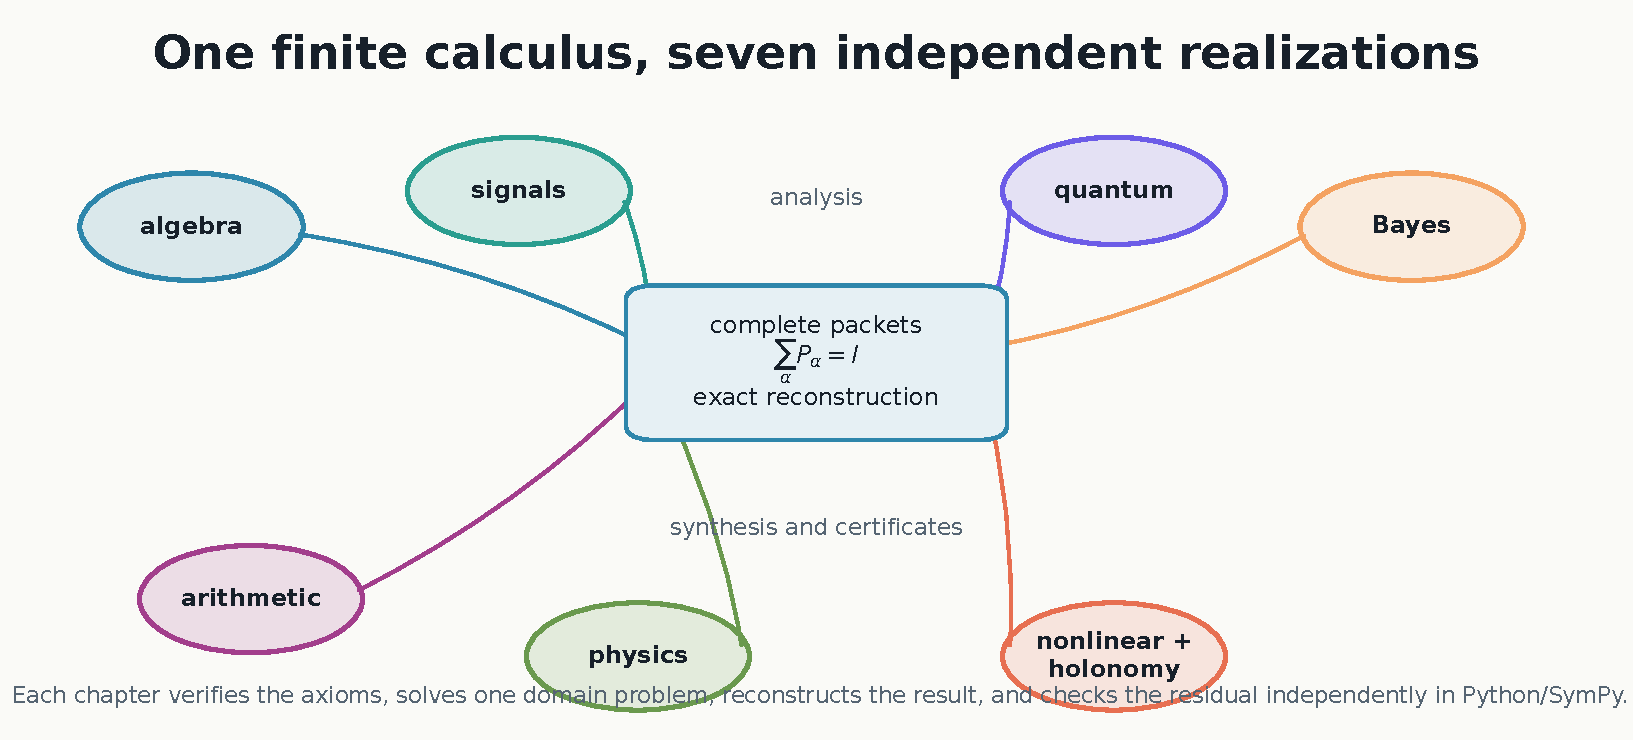
\includegraphics[width=.96\linewidth]{00_cross_domain_pipeline.pdf}
\caption{The common finite calculus and its seven realizations.}
\label{fig:cross-domain}
\end{figure}

\begin{table}[H]
\centering
\caption{The seven worked areas and their principal exact certificates.}
\begin{tabularx}{\linewidth}{L{1.45in}Y Y}
\toprule
Area & Domain problem & Exact certificate \\
\midrule
Linear algebra & Reconstruct a vector, an operator, and an operator product from blocks & Four zero matrix residuals \\
Signals & Polyphase, Haar, and Fourier representations of one signal & Exact synthesis and projector completeness \\
Quantum & Bell-state preparation and parity path decomposition & Zero path residual and reduced state $I/2$ \\
Probability & Conditional expectation and Bayesian coarsening & Idempotence, sufficiency, and exact defect factorization \\
Arithmetic & Reciprocal root-filter sequence and closed analytic formula & Integer recurrence, hypergeometric identity, composition formula \\
Physics & Two coupled oscillators & Exact ODE solution and conserved packet energies \\
Nonlinear geometry & Nonlinear filter and cycle holonomy & Zero nonlinear residual; designed obstruction norm $8/5$ \\
\bottomrule
\end{tabularx}
\end{table}

% BEGIN INLINED core_to_areas.tex
\chapter{The transfer algebra as a genuine calculus}\label{ch:transfer-calculus}

\section{The block representation is an algebra isomorphism}
The finite realization theorem reconstructs each operator from its transfer blocks.  The stronger statement is that the complete family of blocks is an exact coordinate representation of the entire operator algebra.

Let
\[
\mathfrak B_{\mathcal P}
=
\bigoplus_{\alpha,\beta}
\operatorname{Hom}(X_\alpha,X_\beta).
\]
Define
\[
\Phi_{\mathcal P}:\operatorname{End}(X)\longrightarrow\mathfrak B_{\mathcal P},
\qquad
\Phi_{\mathcal P}(T)=(P_\beta TP_\alpha)_{\beta,\alpha}.
\]
Equip $\mathfrak B_{\mathcal P}$ with matrix-style multiplication
\[
(B\star C)_{\gamma\alpha}
=
\sum_\beta B_{\gamma\beta}C_{\beta\alpha}.
\]

\begin{theorem}[Full block-algebra representation]\label{thm:block-algebra-iso}
$\Phi_{\mathcal P}$ is a unital algebra isomorphism.  Its inverse is
\[
\boxed{
\Phi_{\mathcal P}^{-1}((B_{\beta\alpha}))
=
\sum_{\alpha,\beta}B_{\beta\alpha}.
}
\]
\end{theorem}

\begin{proof}
Exact operator reconstruction proves that the displayed inverse recovers $T$.  Conversely, if each $B_{\beta\alpha}$ maps $X_\alpha$ into $X_\beta$, then
\[
P_\delta\left(\sum_{\alpha,\beta}B_{\beta\alpha}\right)P_\gamma
=B_{\delta\gamma}
\]
because all other corners are annihilated.  The block multiplication theorem gives
\[
\Phi_{\mathcal P}(ST)=\Phi_{\mathcal P}(S)\star\Phi_{\mathcal P}(T).
\]
The identity operator corresponds to the diagonal block identity.
\end{proof}

\section{Support graphs and packet paths}
Define the support relation
\[
\alpha\longrightarrow\beta
\quad\Longleftrightarrow\quad
P_\beta TP_\alpha\ne0.
\]
This produces a directed transfer graph.  The graph records possible movement, while the blocks retain the exact linear maps and weights.

\begin{theorem}[Path expansion for powers]\label{thm:path-power}
For every $m\ge1$,
\[
\boxed{
P_{\alpha_m}T^mP_{\alpha_0}
=
\sum_{\alpha_1,\ldots,\alpha_{m-1}}
(P_{\alpha_m}TP_{\alpha_{m-1}})\cdots
(P_{\alpha_1}TP_{\alpha_0}).
}
\]
Only directed packet paths contribute nonzero terms.
\end{theorem}

\begin{proof}
Insert $I=\sum_\alpha P_\alpha$ between every adjacent pair of copies of $T$ and distribute.  Pairwise annihilation removes every incompatible path.
\end{proof}

\section{The master transfer operator}
Return to the cyclic seed example and define
\[
T=2I-U+3U^2.
\]
In the coordinate basis,
\[
T=
\begin{pmatrix}
2&0&0&0&0&0&3&-1\\
-1&2&0&0&0&0&0&3\\
3&-1&2&0&0&0&0&0\\
0&3&-1&2&0&0&0&0\\
0&0&3&-1&2&0&0&0\\
0&0&0&3&-1&2&0&0\\
0&0&0&0&3&-1&2&0\\
0&0&0&0&0&3&-1&2
\end{pmatrix}.
\]
Applying it to
\[
x=(2,-1,3,0,1,4,-2,5)^{\mathsf T}
\]
gives
\[
\boxed{
Tx=(-7,11,13,-6,11,7,-5,24)^{\mathsf T}.
}
\]

\begin{calculationbox}[ coordinate rule]
Because $(Ux)_j=x_{j-1}$ and $(U^2x)_j=x_{j-2}$ with indices modulo eight,
\[
(Tx)_j=2x_j-x_{j-1}+3x_{j-2}.
\]
For example,
\[
(Tx)_0=2(2)-x_7+3x_6=4-5-6=-7,
\]
and
\[
(Tx)_7=2(5)-x_6+3x_5=10+2+12=24.
\]
\end{calculationbox}

\SafeFigure[.78\linewidth]{45_transfer_support_matrix.pdf}{The exact support pattern of the transfer blocks.  A nonzero cell records a genuine packet-to-packet map, not merely a correlation.}{fig:master-transfer-support}

\SafeFigure[.96\linewidth]{55_master_seed_and_transfer_output.pdf}{The generated object and the exact output of the declared transfer operator.}{fig:master-transfer-output}

\section{Composition with a second operator}
Let
\[
S=I+U^3.
\]
The product $ST$ may be calculated directly, but the calculus resolves it through every intermediate address:
\[
P_bSTP_a
=
\sum_{\gamma=0}^{7}
(P_bSP_\gamma)(P_\gamma TP_a).
\]
Summing over $a$ and $b$ reconstructs $ST$ exactly.

\SafeFigure[.96\linewidth]{47_operator_path_sum.pdf}{A reduced visualization of the packet-path law.  The proof sums all intermediate addresses, including paths that vanish.}{fig:master-path-sum}

\begin{certificate}[ master product]
The symbolic matrix
\[
\sum_{a,b,\gamma}
E_bSE_\gamma TE_a-ST
\]
is exactly the zero $8\times8$ matrix.
\end{certificate}

\section{Adjoints, symmetries, and diagonalization}
When the packets are orthogonal,
\[
(P_\beta TP_\alpha)^*=P_\alpha T^*P_\beta.
\]
Thus adjunction reverses every transfer edge.  If $T$ commutes with every packet projector, all off-diagonal blocks vanish and the packets reduce $T$.

For the cyclic operator $T=2I-U+3U^2$, the Fourier transform diagonalizes $U$ and hence diagonalizes $T$.  If $FUF^*=\diag(\zeta_0,\ldots,\zeta_7)$, then
\[
FTF^*
=
\diag(2-\zeta_k+3\zeta_k^2)_{k=0}^{7}.
\]
The operator is banded in spatial coordinates and diagonal in Fourier coordinates.

\SafeFigure[.96\linewidth]{46_operator_spatial_fourier.pdf}{The same operator in the spatial and Fourier atlases.  Coordinate transport changes the matrix pattern but not the underlying map.}{fig:master-operator-atlases}

\begin{stepbox}{Seed-to-finish Step 7: transfer blocks}
Insert complete projectors on both sides of the operator.  The resulting block field is an exact operator coordinate system.
\end{stepbox}

\begin{stepbox}{Seed-to-finish Step 8: packet paths}
Insert complete projectors between composed operators.  Products, powers, circuits, and time steps become exact sums over packet paths.
\end{stepbox}

\chapter{Refinement, coarsening, and multiple atlases}\label{ch:refinement-atlases}

\section{Coordinate refinement maps}
Let $\mathcal P=\{P_\alpha\}$ be coarse and $\mathcal Q=\{Q_\rho\}$ be fine, with
\[
P_\alpha=\sum_{\rho\succ\alpha}Q_\rho.
\]
Both packet tuples are exact coordinate copies of $X$.  Define
\[
J=\Acal_{\mathcal Q}\Scal_{\mathcal P},
\qquad
C=\Acal_{\mathcal P}\Scal_{\mathcal Q}.
\]

\begin{theorem}[Exact coordinate refinement]\label{thm:coordinate-refinement}
On the direct sums of the actual packet ranges,
\[
\boxed{CJ=I_{\oplus X_\alpha},\qquad JC=I_{\oplus Y_\rho}.}
\]
Thus refinement and coarsening are inverse coordinate changes when all children are retained.
\end{theorem}

\begin{proof}
Use exact analysis and synthesis at each level:
\[
CJ
=
\Acal_{\mathcal P}\Scal_{\mathcal Q}
\Acal_{\mathcal Q}\Scal_{\mathcal P}
=
\Acal_{\mathcal P}I_X\Scal_{\mathcal P}
=I.
\]
The proof of $JC=I$ is identical.
\end{proof}

\begin{remark}
Refinement is not truncation.  Loss begins only when a child packet is discarded, merged through a noninvertible statistic, or replaced by a model.
\end{remark}

\SafeFigure[.82\linewidth]{48_refinement_incidence.pdf}{The exact parent-child incidence for the parity-to-mod-four refinement.}{fig:refinement-incidence}

\section{The master refinement}
The parity packets refine into mod-four packets, which refine into coordinate packets:
\[
P_{\mathrm e}=R_0+R_2,
\qquad
P_{\mathrm o}=R_1+R_3,
\]
\[
R_r=E_r+E_{r+4}.
\]
Therefore
\[
P_{\mathrm e}x
=
E_0x+E_2x+E_4x+E_6x,
\]
and similarly for the odd packet.  Every equality is exact over $\C^8$.

\section{Transfer blocks under refinement}
Refining both the source and target packets gives
\[
P_\beta TP_\alpha
=
\sum_{\sigma\succ\beta}
\sum_{\rho\succ\alpha}
Q_\sigma TQ_\rho.
\]
The coarse block is not replaced by a different operator.  It is exactly reconstructed from the fine child blocks.

For a weighted filtration, assign a nonnegative weight $w(\beta,\alpha)$ to each transfer edge and define the weight of a path as the sum of its edge weights.  Truncation by total weight then has an explicit omitted-path residual.  The exact block and path formulas remain prior to any truncation.

\section{Transform atlases and pulled-back projectors}
Let $U:X\to Y$ be invertible and let $E_\alpha$ be the ordinary coordinate projectors on $Y$.  The pulled-back projectors
\[
P_\alpha=U^{-1}E_\alpha U
\]
form a complete atlas on $X$.  The signal chapter later takes $U$ to be Fourier and Haar transforms; the physics chapter takes $U$ to be the normal-mode transform; the quantum chapter takes $U$ to be a basis-changing unitary.

\SafeFigure[.96\linewidth]{49_transform_atlas_portfolio.pdf}{Spatial, Fourier, Haar, and general conjugated packet systems are exact atlases of one object.}{fig:atlas-portfolio}

\section{A redundant exact multi-atlas frame}
Several complete unitary atlases may be retained simultaneously.  Let $U_1,\ldots,U_m$ be unitary and let $w_a>0$.  Define
\[
\Acal x=(w_aU_ax)_{a=1}^m.
\]

\begin{theorem}[Weighted multi-atlas reconstruction]\label{thm:multi-atlas}
The canonical synthesis
\[
\Scal((c_a)_a)
=
\frac{1}{W}
\sum_{a=1}^m w_aU_a^*c_a,
\qquad
W=\sum_{a=1}^m w_a^2,
\]
satisfies
\[
\boxed{\Scal\Acal=I_X.}
\]
Moreover,
\[
\sum_{a=1}^m\|w_aU_ax\|^2=W\|x\|^2.
\]
\end{theorem}

\begin{proof}
Unitary inversion gives
\[
\Scal\Acal x
=
\frac1W\sum_aw_a^2U_a^*U_ax
=
\frac1W\sum_aw_a^2x=x.
\]
The energy identity follows from $\|U_ax\|=\|x\|$.
\end{proof}

For the master vector, choose
\[
U_1=I,
\qquad
U_2=F,
\qquad
U_3=H,
\qquad
(w_1,w_2,w_3)=(1,2,3).
\]
Then $W=14$ and
\[
\widehat x
=
\frac1{14}
\left(c_1+2F^*c_2+3H^*c_3\right)
=x.
\]

\SafeFigure[.96\linewidth]{50_multi_atlas_tight_frame.pdf}{The master spatial-Fourier-Haar portfolio is redundant but exactly reconstructing.}{fig:multi-atlas-frame}

\section{Completion direction}
A refinement tower
\[
\mathcal P^{(0)}\prec\mathcal P^{(1)}\prec\cdots
\]
is algebraically coherent when every parent is the sum of its children.  In a finite object this tower terminates.  In an infinite object one must additionally declare a topology or inverse-limit structure and prove convergence.

\SafeFigure[.95\linewidth]{53_completion_refinement_tower.pdf}{The finite master tower.  The figure also marks the additional datum needed in an infinite theory: a declared convergence structure.}{fig:completion-tower}

\begin{stepbox}{Seed-to-finish Step 9: refinement}
Replace a packet by a complete child family.  Because all children are retained, refinement is an invertible coordinate change.
\end{stepbox}

\begin{stepbox}{Seed-to-finish Step 10: atlas portfolio}
Transport ordinary coordinate projectors through Fourier, wavelet, modal, or other invertible transforms.  Several unitary atlases may be retained together through the exact tight-frame synthesis theorem.
\end{stepbox}

\chapter{Nonlinear packets, obstruction packets, and completion}\label{ch:nonlinear-completion}

\section{Exact nonlinear packet coordinates}
Let $N:X\to Y$ be an arbitrary map between finite spaces with complete packet systems $\mathcal P$ on $X$ and $\mathcal Q$ on $Y$.  Define the packet-coordinate map
\[
\widetilde N
=
\Acal_{\mathcal Q}N\Scal_{\mathcal P}.
\]

\begin{theorem}[Exact nonlinear conjugacy]\label{thm:nonlinear-conjugacy}
The nonlinear map is recovered exactly by
\[
\boxed{
N
=
\Scal_{\mathcal Q}\widetilde N\Acal_{\mathcal P}.
}
\]
No linearity assumption on $N$ is required.
\end{theorem}

\begin{proof}
Use $\Scal_{\mathcal Q}\Acal_{\mathcal Q}=I_Y$ and $\Scal_{\mathcal P}\Acal_{\mathcal P}=I_X$:
\[
\Scal_{\mathcal Q}\widetilde N\Acal_{\mathcal P}
=
\Scal_{\mathcal Q}\Acal_{\mathcal Q}
N
\Scal_{\mathcal P}\Acal_{\mathcal P}
=N.
\]
\end{proof}

The theorem says that nonlinear packet coordinates are exact, but it does not say that packets evolve independently.  Nonlinearity creates interactions among input packets.

\section{Multilinear interaction tensors}
Let $B:X\times X\to Y$ be bilinear.  Since $x=\sum_aP_ax$,
\[
\boxed{
B(x,x)
=
\sum_{a,c}B(P_ax,P_cx).
}
\]
Resolving the output gives
\[
B_{b;ac}(x)
=
Q_bB(P_ax,P_cx),
\]
which is a three-index interaction tensor rather than a two-index transfer matrix.

More generally, for a $k$-linear map $M$,
\[
Q_bM(x_1,\ldots,x_k)
=
\sum_{a_1,\ldots,a_k}
Q_bM(P_{a_1}x_1,\ldots,P_{a_k}x_k).
\]

\SafeFigure[.93\linewidth]{51_nonlinear_interaction_hypergraph.pdf}{Linear transfer edges become nonlinear interaction hyperedges indexed by several input packets and one output packet.}{fig:nonlinear-hypergraph}

\section{Packet jets}
If $N$ is $k$ times differentiable, its $k$th derivative is a $k$-linear map.  Therefore
\[
\boxed{
Q_bD^kN(x)[h_1,\ldots,h_k]
=
\sum_{a_1,\ldots,a_k}
Q_bD^kN(x)[P_{a_1}h_1,\ldots,P_{a_k}h_k].
}
\]
The complete family of these tensors is the packet jet.  Ordinary Taylor expansion may then be written packet by packet without changing its sum.

For a quadratic fixed-point equation
\[
x=s+B(x,x),
\]
repeated substitution produces rooted binary trees.  Each leaf carries a seed packet, each internal vertex carries a bilinear interaction block, and synthesis sums all packet-labeled trees.  Convergence is an analytic question; the packet labeling itself is exact at every finite order.

\section{The master nonlinear map}
Define
\[
N(x)=x+(Ux)\odot(U^3x),
\]
where $\odot$ is coordinatewise multiplication.  For the master vector,
\[
\boxed{
N(x)=(22,-5,-2,6,1,7,-2,3)^{\mathsf T}.
}
\]

\begin{calculationbox}[ first coordinate]
Because $(Ux)_0=x_7=5$ and $(U^3x)_0=x_5=4$,
\[
N(x)_0=x_0+(Ux)_0(U^3x)_0=2+5\cdot4=22.
\]
Every remaining coordinate follows the same cyclic rule.
\end{calculationbox}

The bilinear term resolves exactly as
\[
(Ux)\odot(U^3x)
=
\sum_{a,c}
(UE_ax)\odot(U^3E_cx).
\]
The symbolic residual is the zero vector.

\SafeFigure[.94\linewidth]{57_master_nonlinear_reconstruction.pdf}{The master input and nonlinear output.  The full output is synthesized from exact interaction packets.}{fig:master-nonlinear-output}

\section{Obstruction packets}
Packet coordinates can expose a failure without guaranteeing that it vanishes.  Let $L:H\to K$ be a linear map between finite-dimensional inner-product spaces.  Let $L^\dagger$ be its Moore--Penrose inverse and define
\[
\Pi_{\mathrm{Obs}}=I-LL^\dagger.
\]

\begin{theorem}[Finite obstruction criterion]\label{thm:obstruction-criterion}
The equation
\[
Lh=d
\]
is solvable if and only if
\[
\boxed{\Pi_{\mathrm{Obs}}d=0.}
\]
The obstruction packet is the orthogonal projection of $d$ onto $\Ran(L)^\perp$.
\end{theorem}

\begin{proof}
$LL^\dagger$ is the orthogonal projector onto $\Ran(L)$.  Thus $I-LL^\dagger$ projects onto the orthogonal complement.  The vector $d$ lies in the range exactly when its complementary projection vanishes.
\end{proof}

Take
\[
L=
\begin{pmatrix}
1&0\\0&1\\1&1
\end{pmatrix}.
\]
Then
\[
\Pi_{\mathrm{Obs}}
=
\frac13
\begin{pmatrix}
1&1&-1\\
1&1&-1\\
-1&-1&1
\end{pmatrix}.
\]
For $d=(1,2,3)^{\mathsf T}$ the obstruction is zero.  For
\[
d'=(1,2,4)^{\mathsf T},
\]
\[
\boxed{
\Pi_{\mathrm{Obs}}d'
=
\left(-\frac13,-\frac13,\frac13\right)^{\mathsf T}\ne0.
}
\]

\SafeFigure[.96\linewidth]{52_obstruction_packet_geometry.pdf}{Positive and negative controls for the finite obstruction theorem.  The nonzero packet localizes the exact failed compatibility condition.}{fig:obstruction-geometry}

\section{Completion from a dense core}
The finite theorems extend to completed spaces only under explicit continuity hypotheses.

\begin{theorem}[Dense-core extension]\label{thm:dense-extension}
Let $X$ be a normed space, let $D\subseteq X$ be dense, and let $A,B:X\to Y$ be bounded linear maps into a normed space $Y$.  If $Ax=Bx$ for every $x\in D$, then $A=B$ on $X$.
\end{theorem}

\begin{proof}
For $x\in X$, choose $x_n\in D$ with $x_n\to x$.  Boundedness gives
\[
Ax=\lim_nAx_n=\lim_nBx_n=Bx.
\]
\end{proof}

\begin{corollary}[Completion preserves a finite packet split]\label{cor:packet-completion}
Suppose bounded operators $P_1,\ldots,P_m$ satisfy
\[
P_iP_j=\delta_{ij}P_i,
\qquad
\sum_iP_i=I
\]
on a dense invariant subspace $D$.  Then the same identities hold on the completion of $D$.
\end{corollary}

\begin{proof}
Every difference between the two sides is a bounded operator vanishing on $D$, so apply \cref{thm:dense-extension}.
\end{proof}

\begin{boundarybox}[ infinite towers]
An inverse system of exact finite reconstructions does not automatically produce a nonempty, complete, or physically meaningful limit.  One must prove compatibility, completeness, domain preservation, and convergence in the declared topology.
\end{boundarybox}

\begin{stepbox}{Seed-to-finish Step 11: nonlinear interaction}
Replace transfer matrices by interaction tensors or trees.  Analysis and synthesis remain exact even though packet independence generally fails.
\end{stepbox}

\begin{stepbox}{Seed-to-finish Step 12: obstruction}
Project a continuation defect onto the complement of the correction range.  Vanishing is the exact solvability criterion; nonvanishing is retained as a localized packet rather than hidden.
\end{stepbox}

\begin{stepbox}{Seed-to-finish Step 13: completion}
Pass from a dense finite or algebraic core only after the relevant projectors and operators are proved bounded or otherwise controlled on their domains.
\end{stepbox}

\chapter{One seed through the entire calculus}\label{ch:master-example}

\section{The complete step ledger}
This chapter repeats the master cyclic example without skipping any layer.  The purpose is to show that the definitions form one continuous calculus rather than a collection of disconnected identities.

\SafeFigure[.98\linewidth]{54_master_example_pipeline.pdf}{The master example from primitive seed through nonlinear interaction and final reconstruction.}{fig:master-full-pipeline}

\subsection{Step 0: choose the ambient type}
Declare
\[
X=\C^8
\]
with standard basis $e_0,\ldots,e_7$ and the usual Hermitian inner product.  The finite dimension makes all linear operators bounded and all sums finite.

\subsection{Step 1: choose the seed}
Set
\[
s=e_0.
\]
At this stage only one primitive vector has been supplied.

\subsection{Step 2: choose the operator grammar}
Let the grammar be generated by the forward cyclic shift $U$.  The admissible linear operators are polynomials in $U$.

\subsection{Step 3: compute the orbit}
The orbit is
\[
\{s,Us,\ldots,U^7s\}
=
\{e_0,e_1,\ldots,e_7\}.
\]
The orbit matrix has rank eight, so one seed generates all of $X$.

\subsection{Step 4: impose the relation}
The exact relation is
\[
U^8=I.
\]
Hence every operator word has a unique normal form of degree at most seven.

\subsection{Step 5: generate the object}
Use
\[
p(z)=2-z+3z^2+z^4+4z^5-2z^6+5z^7
\]
and form
\[
x=p(U)s=(2,-1,3,0,1,4,-2,5)^{\mathsf T}.
\]

\subsection{Step 6: declare the packet addresses}
Use four exact atlases:
\begin{enumerate}[label=(\alph*),leftmargin=2em]
\item coordinate packets $E_j$;
\item parity packets $P_{\mathrm e},P_{\mathrm o}$;
\item mod-four packets $R_0,\ldots,R_3$;
\item Fourier character packets $Q_0,\ldots,Q_7$.
\end{enumerate}
Each family is complete at its own level.

\subsection{Step 7: analyze and synthesize}
Coordinate analysis gives
\[
\Acal_E x=(E_0x,\ldots,E_7x),
\]
and
\[
\Scal_E\Acal_E x
=
\sum_{j=0}^7E_jx=x.
\]
The exact residual is zero.

\subsection{Step 8: declare a transfer operator}
Set
\[
T=2I-U+3U^2.
\]
The output is
\[
Tx=(-7,11,13,-6,11,7,-5,24)^{\mathsf T}.
\]

\subsection{Step 9: reconstruct the operator}
Resolve
\[
T_{ba}=E_bTE_a.
\]
Then
\[
\sum_{a,b}T_{ba}=T.
\]
The support graph has exactly the cyclic identity, one-step, and two-step bands dictated by the polynomial in $U$.

\subsection{Step 10: compose by paths}
Let $S=I+U^3$.  The product is reconstructed from
\[
E_bSTE_a
=
\sum_\gamma(E_bSE_\gamma)(E_\gamma TE_a).
\]
The complete path-sum residual is zero.

\subsection{Step 11: refine}
Use
\[
P_{\mathrm e}=R_0+R_2,
\qquad
P_{\mathrm o}=R_1+R_3,
\]
and
\[
R_r=E_r+E_{r+4}.
\]
Every coarse object packet and every coarse operator block is recovered by summing its fine descendants.

\subsection{Step 12: transport to Fourier space}
Let $F$ be the unitary DFT.  The projectors
\[
Q_k=F^*E_kF
\]
are complete, mutually annihilating, and idempotent.  In this atlas,
\[
FTF^*
=
\diag(2-\zeta_k+3\zeta_k^2).
\]

\SafeFigure[.89\linewidth]{56_master_fourier_packets.pdf}{The exact Fourier magnitudes and phases of the master vector.  Both are required for complete synthesis.}{fig:master-fourier-packets}

\subsection{Step 13: retain several atlases simultaneously}
Analyze $x$ through spatial, Fourier, and Haar transforms with weights $(1,2,3)$.  The canonical tight-frame synthesis divides by
\[
1^2+2^2+3^2=14
\]
and reconstructs $x$ exactly.

\subsection{Step 14: apply a nonlinear operation}
Use
\[
N(x)=x+(Ux)\odot(U^3x).
\]
The output interaction sum over all packet pairs equals the direct nonlinear term, and output synthesis returns
\[
N(x)=(22,-5,-2,6,1,7,-2,3)^{\mathsf T}.
\]

\subsection{Step 15: test an obstruction}
For the separate continuation map
\[
L=\begin{pmatrix}1&0\\0&1\\1&1\end{pmatrix},
\]
the datum $(1,2,3)^{\mathsf T}$ has zero obstruction and is solvable.  The datum $(1,2,4)^{\mathsf T}$ has obstruction
\[
\left(-\frac13,-\frac13,\frac13\right)^{\mathsf T},
\]
so no exact correction exists in the declared range.

\subsection{Step 16: close the reconstruction loop}
The exact symbolic certificates are
\[
\begin{array}{ll}
\rank\mathcal O_U(s)=8,&U^8-I=0,\\[2pt]
\sum_jE_jx-x=0,&\sum_{a,b}E_bTE_a-T=0,\\[2pt]
\sum_{a,b,\gamma}E_bSE_\gamma TE_a-ST=0,&\sum_kQ_k-I=0,\\[2pt]
\Scal\Acal x-x=0,&\sum_bE_bN(x)-N(x)=0.
\end{array}
\]
The intended negative control is the nonzero blocked obstruction.

\SafeFigure[.95\linewidth]{58_master_certificate_dashboard.pdf}{The master certificate ledger.  The nonzero obstruction row is intentionally retained because a calculus must detect failures as well as exact reconstructions.}{fig:master-dashboard}

\section{Complete symbolic implementation}
\begin{lstlisting}
from proof_atlas.foundations import build_certificate, matrix_zero

c = build_certificate()
assert c.orbit_rank == 8
assert matrix_zero(c.relation_residual)
assert matrix_zero(c.spatial_reconstruction_residual)
assert matrix_zero(c.transfer_reconstruction_residual)
assert matrix_zero(c.product_path_residual)
assert matrix_zero(c.fourier_completeness_residual)
assert matrix_zero(c.multi_atlas_reconstruction_residual)
assert matrix_zero(c.nonlinear_packet_residual)
assert matrix_zero(c.bilinear_interaction_residual)
assert matrix_zero(c.solvable_obstruction)
assert not matrix_zero(c.blocked_obstruction)
\end{lstlisting}

\chapter{The start-to-finish realization theorem}\label{ch:start-finish-theorem}

\section{Statement}
The preceding chapters can now be assembled into one dependency-ordered theorem.

\begin{theorem}[Finite seed-to-reconstruction theorem]\label{thm:seed-to-reconstruction}
Let $X$ be finite-dimensional.  Suppose the following data are declared:
\begin{enumerate}[label=(\roman*),leftmargin=2em]
\item a finite seed family $S$;
\item a fixed unital operator algebra $\mathcal A\subseteq\operatorname{End}(X)$;
\item a relation system presenting the generated hull;
\item one or more complete packet atlases;
\item exact refinement maps among selected atlases;
\item an admissible linear, multilinear, polynomial, or arbitrary finite map;
\item a synthesis law for every retained coordinate family.
\end{enumerate}
Then:
\begin{enumerate}[label=(\alph*),leftmargin=2em]
\item the generated object lies in the quotient of the free seed module by the relation kernel;
\item every complete atlas reconstructs the object exactly;
\item every linear operator reconstructs from its transfer blocks;
\item operator products reconstruct from packet paths;
\item complete refinement preserves both object and operator reconstruction;
\item arbitrary nonlinear maps possess exact packet-coordinate conjugates;
\item multilinear terms decompose into complete interaction tensors;
\item finite correction problems admit exact obstruction packets;
\item every bounded identity established on a dense invariant core extends to its completion;
\item every final equality has an explicit object-level or operator-level residual certificate.
\end{enumerate}
\end{theorem}

\begin{proof}
Part (a) is \cref{thm:seed-presentation}.  Parts (b) and (c) are the object and operator reconstruction theorems.  Part (d) follows from repeated insertion of packet completeness.  Part (e) is \cref{thm:coordinate-refinement} and the refined-block identity.  Part (f) is \cref{thm:nonlinear-conjugacy}; part (g) follows by multilinearity.  Part (h) is \cref{thm:obstruction-criterion}.  Part (i) is \cref{thm:dense-extension,cor:packet-completion}.  The residual in part (j) is obtained by subtracting the reconstructed quantity from the direct quantity at the appropriate type.
\end{proof}

\SafeFigure[.92\linewidth]{60_theorem_dependency_ladder.pdf}{Each theorem depends on the preceding layers.  The cross-domain examples come after, not before, this proof chain.}{fig:dependency-ladder}

\section{Why the construction deserves the name calculus}
The term calculus is justified by closure under the recurring operations:
\begin{itemize}[leftmargin=1.6em]
\item seeds generate controlled hulls;
\item relations reduce operator words to normal forms;
\item projectors provide exact coordinate differentials in the broad sense of resolving variation by packet;
\item transfer blocks compose by a matrix law;
\item refinement has exact chain maps and inverse synthesis;
\item nonlinear maps possess packet jets and interaction trees;
\item obstructions localize failed continuation;
\item completion transports finite identities under declared continuity hypotheses;
\item synthesis returns every retained calculation to the original object space.
\end{itemize}
These operations are not one isolated theorem.  They form a closed grammar for constructing, resolving, transforming, refining, and reconstructing mathematical objects.

\SafeFigure[.72\linewidth]{59_complete_calculus_wheel.pdf}{The operational cycle of the calculus.  Reconstruction is not the end: the residual may become the seed for the next refinement.}{fig:calculus-wheel}

\section{Transition to the seven independent realizations}
The master example proves the entire chain in one finite cyclic module.  The next seven chapters retain all of their original content and repeat the verification in different domains.  Their role is to show that the common theorem is not tied to the cyclic shift example:
\begin{enumerate}[label=\arabic*.,leftmargin=2em]
\item a general rational matrix decomposition;
\item signal polyphase, Fourier, and wavelet coordinates;
\item quantum circuit paths and reduced states;
\item conditional expectation and Bayesian information loss;
\item closed analytic and arithmetic coefficient families;
\item physical normal modes and conserved energy;
\item nonlinear filters and geometric holonomy.
\end{enumerate}
% END INLINED core_to_areas.tex

\part{Seven Worked Areas}

\chapter{Area I: finite linear algebra and exact transfer blocks}\label{ch:linear}

\section{Problem}
Resolve a concrete vector and a concrete operator in $\Q^6$ into three two-dimensional packets, prove exact reconstruction, prove the block product law on a second operator, and refine one packet into one-dimensional children.

\section{Step 1: declare the projectors}
Partition the coordinate positions as
\[
X_0=\operatorname{span}(e_1,e_2),\qquad
X_1=\operatorname{span}(e_3,e_4),\qquad
X_2=\operatorname{span}(e_5,e_6).
\]
The projectors are
\[
P_0=\diag(1,1,0,0,0,0),
\quad
P_1=\diag(0,0,1,1,0,0),
\quad
P_2=\diag(0,0,0,0,1,1).
\]
They visibly satisfy
\[
P_iP_j=\delta_{ij}P_i,
\qquad P_0+P_1+P_2=I_6.
\]

\section{Step 2: decompose and reconstruct the object}
Take
\[
x=(2,-1,3,4,-2,5)^{\mathsf T}.
\]
Then
\[
\begin{aligned}
P_0x&=(2,-1,0,0,0,0)^{\mathsf T},\\
P_1x&=(0,0,3,4,0,0)^{\mathsf T},\\
P_2x&=(0,0,0,0,-2,5)^{\mathsf T}.
\end{aligned}
\]
Adding gives $x$ exactly.

\begin{calculationbox}[ for object synthesis]
The coordinate sum can be checked entry by entry:
\[
\begin{array}{c|rrrrrr}
&1&2&3&4&5&6\\
\hline
P_0x&2&-1&0&0&0&0\\
P_1x&0&0&3&4&0&0\\
P_2x&0&0&0&0&-2&5\\
\hline
\sum_iP_ix&2&-1&3&4&-2&5
\end{array}
\]
The important point is that the zero pattern is forced by the projectors. No coordinate is counted twice and no coordinate is omitted.
\end{calculationbox}

\SafeFigure[.94\linewidth]{20_linear_object_packets.pdf}{The vector before and after packet analysis. The three packet vectors have disjoint supports and sum coordinatewise to the original vector.}{fig:linear-object-packets}

\section{Step 3: resolve the operator}
Let
\[
T=
\begin{pmatrix}
1&2&0&0&1&0\\
0&1&1&0&0&1\\
2&0&1&1&0&0\\
0&1&0&2&1&0\\
1&0&0&1&2&1\\
0&0&1&0&0&3
\end{pmatrix}.
\]
In $2\times2$ packet blocks,
\[
[T_{\beta\alpha}]_{\beta,\alpha=0}^2=
\begin{pmatrix}
\begin{psmallmatrix}1&2\\0&1\end{psmallmatrix}&
\begin{psmallmatrix}0&0\\1&0\end{psmallmatrix}&
\begin{psmallmatrix}1&0\\0&1\end{psmallmatrix}\\[4pt]
\begin{psmallmatrix}2&0\\0&1\end{psmallmatrix}&
\begin{psmallmatrix}1&1\\0&2\end{psmallmatrix}&
\begin{psmallmatrix}0&0\\1&0\end{psmallmatrix}\\[4pt]
\begin{psmallmatrix}1&0\\0&0\end{psmallmatrix}&
\begin{psmallmatrix}0&1\\1&0\end{psmallmatrix}&
\begin{psmallmatrix}2&1\\0&3\end{psmallmatrix}
\end{pmatrix}.
\]
Summing the nine embedded blocks reproduces $T$ entry by entry.

Applying the operator gives
\[
Tx=(-2,7,11,5,7,18)^{\mathsf T}.
\]
The three output packets are
\[
(-2,7,0,0,0,0)^{\mathsf T},
\quad
(0,0,11,5,0,0)^{\mathsf T},
\quad
(0,0,0,0,7,18)^{\mathsf T}.
\]

The block contributions can be displayed before they are added.  For output packet $X_0$,
\[
\begin{aligned}
T_{00}P_0x&=(0,-1,0,0,0,0)^{\mathsf T},\\
T_{01}P_1x&=(0,3,0,0,0,0)^{\mathsf T},\\
T_{02}P_2x&=(-2,5,0,0,0,0)^{\mathsf T},
\end{aligned}
\]
so their sum is $P_0Tx=(-2,7,0,0,0,0)^{\mathsf T}$.  The other two output packets obey the same rule:
\[
\begin{array}{c|ccc|c}
\text{output}&\text{from }X_0&\text{from }X_1&\text{from }X_2&\text{sum}\\
\hline
X_0&(0,-1)&(0,3)&(-2,5)&(-2,7)\\
X_1&(4,-1)&(7,8)&(0,-2)&(11,5)\\
X_2&(2,0)&(4,3)&(1,15)&(7,18)
\end{array}
\]
where only the two coordinates belonging to the displayed output packet are shown.

\SafeFigure[.96\linewidth]{21_linear_block_contributions.pdf}{Each pair of bars is one output packet. Colored stacks are the three input-to-output contributions, and the diamond marks their exact sum.}{fig:linear-block-contributions}

\begin{figure}[H]
\centering
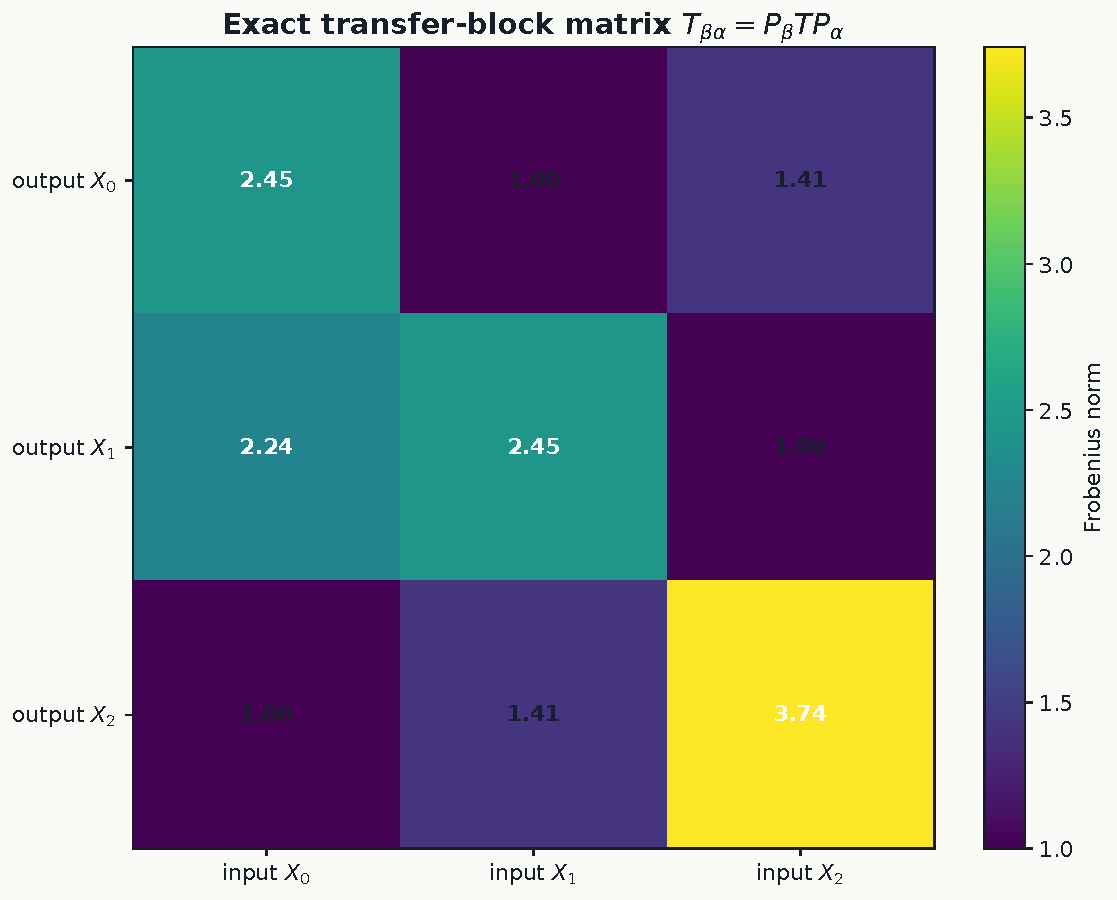
\includegraphics[width=.78\linewidth]{01_linear_transfer_blocks.pdf}
\caption{Norms of the nine exact transfer blocks. The heatmap is a visualization of an exact matrix decomposition, not an approximation.}
\end{figure}

\section{Step 4: multiply operators by packet paths}
Use the explicit second operator
\[
S=
\begin{pmatrix}
2&0&1&0&0&0\\
1&1&0&0&0&1\\
0&1&1&0&1&0\\
0&0&1&1&0&0\\
1&0&0&0&1&1\\
0&1&0&1&0&1
\end{pmatrix}.
\]
For each input packet $\alpha$ and output packet $\gamma$, the code computes
\[
P_\gamma STP_\alpha
-
\sum_{\beta=0}^2(P_\gamma SP_\beta)(P_\beta TP_\alpha).
\]
Every entry is exactly zero. This is a complete finite verification of \cref{thm:block-product} for a nontrivial pair of dense-crossing operators.

One block can be inspected without code.  For input $X_2$ and output $X_0$,
\[
(P_0STP_2)_{X_0\leftarrow X_2}
=
\begin{pmatrix}2&0\\1&4\end{pmatrix}.
\]
The three intermediate packet paths give
\[
\begin{aligned}
(P_0SP_0)(P_0TP_2)&=\begin{pmatrix}2&0\\1&1\end{pmatrix},\\
(P_0SP_1)(P_1TP_2)&=\begin{pmatrix}0&0\\0&0\end{pmatrix},\\
(P_0SP_2)(P_2TP_2)&=\begin{pmatrix}0&0\\0&3\end{pmatrix}.
\end{aligned}
\]
Their sum is exactly the direct block.  This calculation shows what the path index $\beta$ means: it records the packet occupied between $T$ and $S$.

\section{Step 5: refine one packet}
Define
\[
Q_{00}=\diag(1,0,0,0,0,0),
\qquad
Q_{01}=\diag(0,1,0,0,0,0).
\]
Then
\[
\boxed{P_0=Q_{00}+Q_{01}.}
\]
Every coarse block touching $P_0$ is consequently the sum of its child blocks.  For example,
\[
P_2TP_0=P_2TQ_{00}+P_2TQ_{01},
\]
and refining both sides gives
\[
P_0TP_0=
Q_{00}TQ_{00}+Q_{00}TQ_{01}
+Q_{01}TQ_{00}+Q_{01}TQ_{01}.
\]
Thus refinement changes the address resolution of the block matrix, not the represented operator.

\begin{figure}[H]
\centering
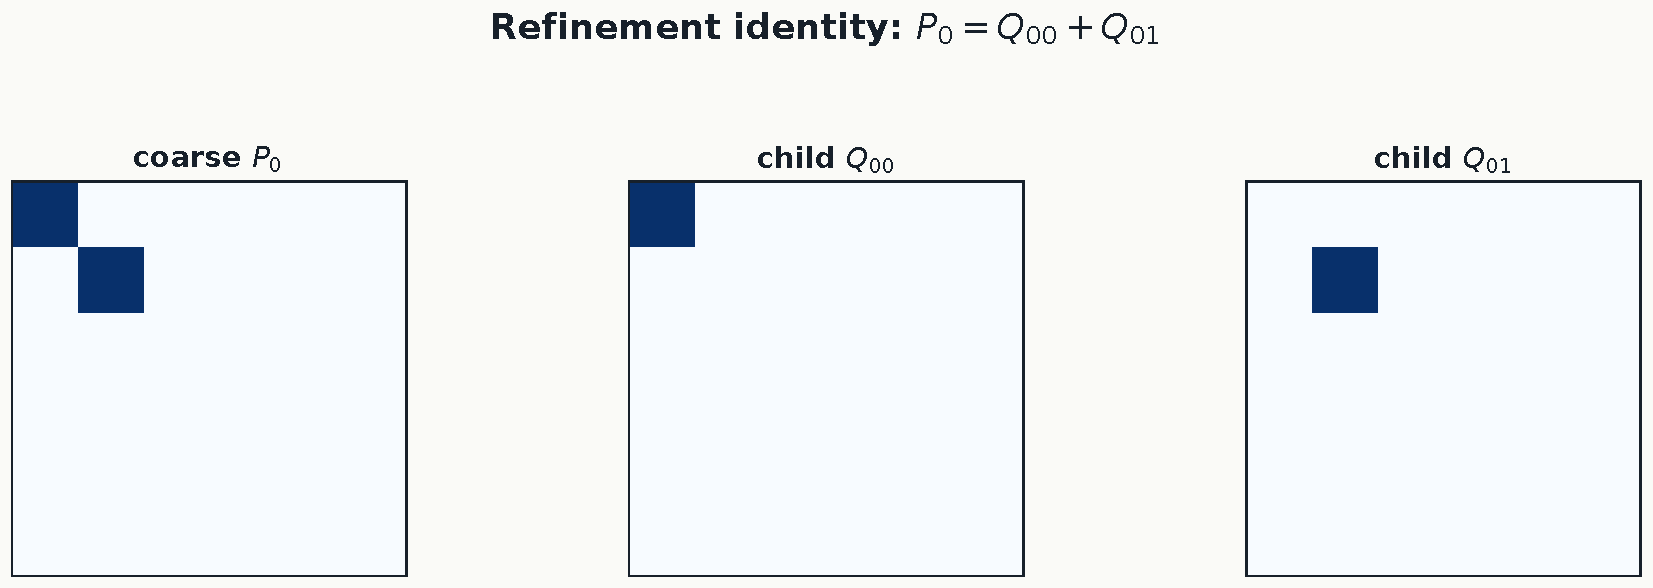
\includegraphics[width=.86\linewidth]{02_linear_refinement.pdf}
\caption{A two-dimensional coordinate packet refined into two one-dimensional descendants.}
\end{figure}

\begin{certificate}
The exact symbolic residuals are
\[
\begin{array}{lr}
\toprule
\text{identity}&\text{residual}\\
\midrule
\sum_iP_ix-x&0_{6\times1}\\
\sum_{i,j}P_iTP_j-T&0_{6\times6}\\
P_\gamma STP_\alpha-\sum_\beta S_{\gamma\beta}T_{\beta\alpha}&0\text{ for all }\gamma,\alpha\\
P_0-Q_{00}-Q_{01}&0_{6\times6}\\
\bottomrule
\end{array}
\]
\end{certificate}

\section{Selected symbolic implementation}
\begin{lstlisting}
P = coordinate_projectors((2, 2, 2))
packets = tuple(Pa * x for Pa in P)
object_residual = sum(packets, sp.zeros(6, 1)) - x

blocks_T = transfer_blocks(T, P)
operator_residual = reconstruct_operator(blocks_T) - T

blocks_ST = transfer_blocks(S * T, P)
product_rebuilt[g][a] = sum(
    blocks_S[g][b] * blocks_T[b][a] for b in range(3)
)
\end{lstlisting}

\chapter{Area II: polyphase, Fourier, and wavelet signal coordinates}\label{ch:signal}

\section{Problem}
Represent one finite signal in residue, polyphase, Haar, and Fourier coordinates; refine the phase system; reconstruct the signal exactly from every complete atlas; and show that Fourier bands are genuine pulled-back projectors.

\section{Step 1: the signal and residue projectors}
Use
\[
x=(3,1,4,1,5,9,2,6)^{\mathsf T}.
\]
For order $N$, define
\[
(P_{N,r}x)[n]=\mathbf1_{n\equiv r\pmod N}x[n].
\]
The projectors satisfy
\[
P_{N,r}P_{N,s}=\delta_{rs}P_{N,r},
\qquad
\sum_{r=0}^{N-1}P_{N,r}=I.
\]

\section{Step 2: exact polyphase analysis and synthesis}
The order-four channels are
\[
\begin{aligned}
x_0&=(3,5)^{\mathsf T},&x_1&=(1,9)^{\mathsf T},\\
x_2&=(4,2)^{\mathsf T},&x_3&=(1,6)^{\mathsf T}.
\end{aligned}
\]
Interleaving them returns
\[
(3,1,4,1,5,9,2,6)^{\mathsf T}=x.
\]

The address rule can be written as a table:
\[
\begin{array}{c|cccccccc}
n&0&1&2&3&4&5&6&7\\
\hline
r=n\bmod4&0&1&2&3&0&1&2&3\\
q=\lfloor n/4\rfloor&0&0&0&0&1&1&1&1\\
x[n]&3&1&4&1&5&9&2&6
\end{array}
\]
Analysis sends the entry at address $n$ to channel $r$ and decimated address $q$.  Synthesis reverses this map by the exact formula
\[
(\Scal_4(x_0,x_1,x_2,x_3))[4q+r]=x_r[q].
\]

\SafeFigure[.98\linewidth]{22_signal_polyphase_interleave.pdf}{Every polyphase coefficient is returned to the unique address $n=4q+r$. The arrows show the complete synthesis map explicitly.}{fig:polyphase-interleave}

\begin{figure}[H]
\centering
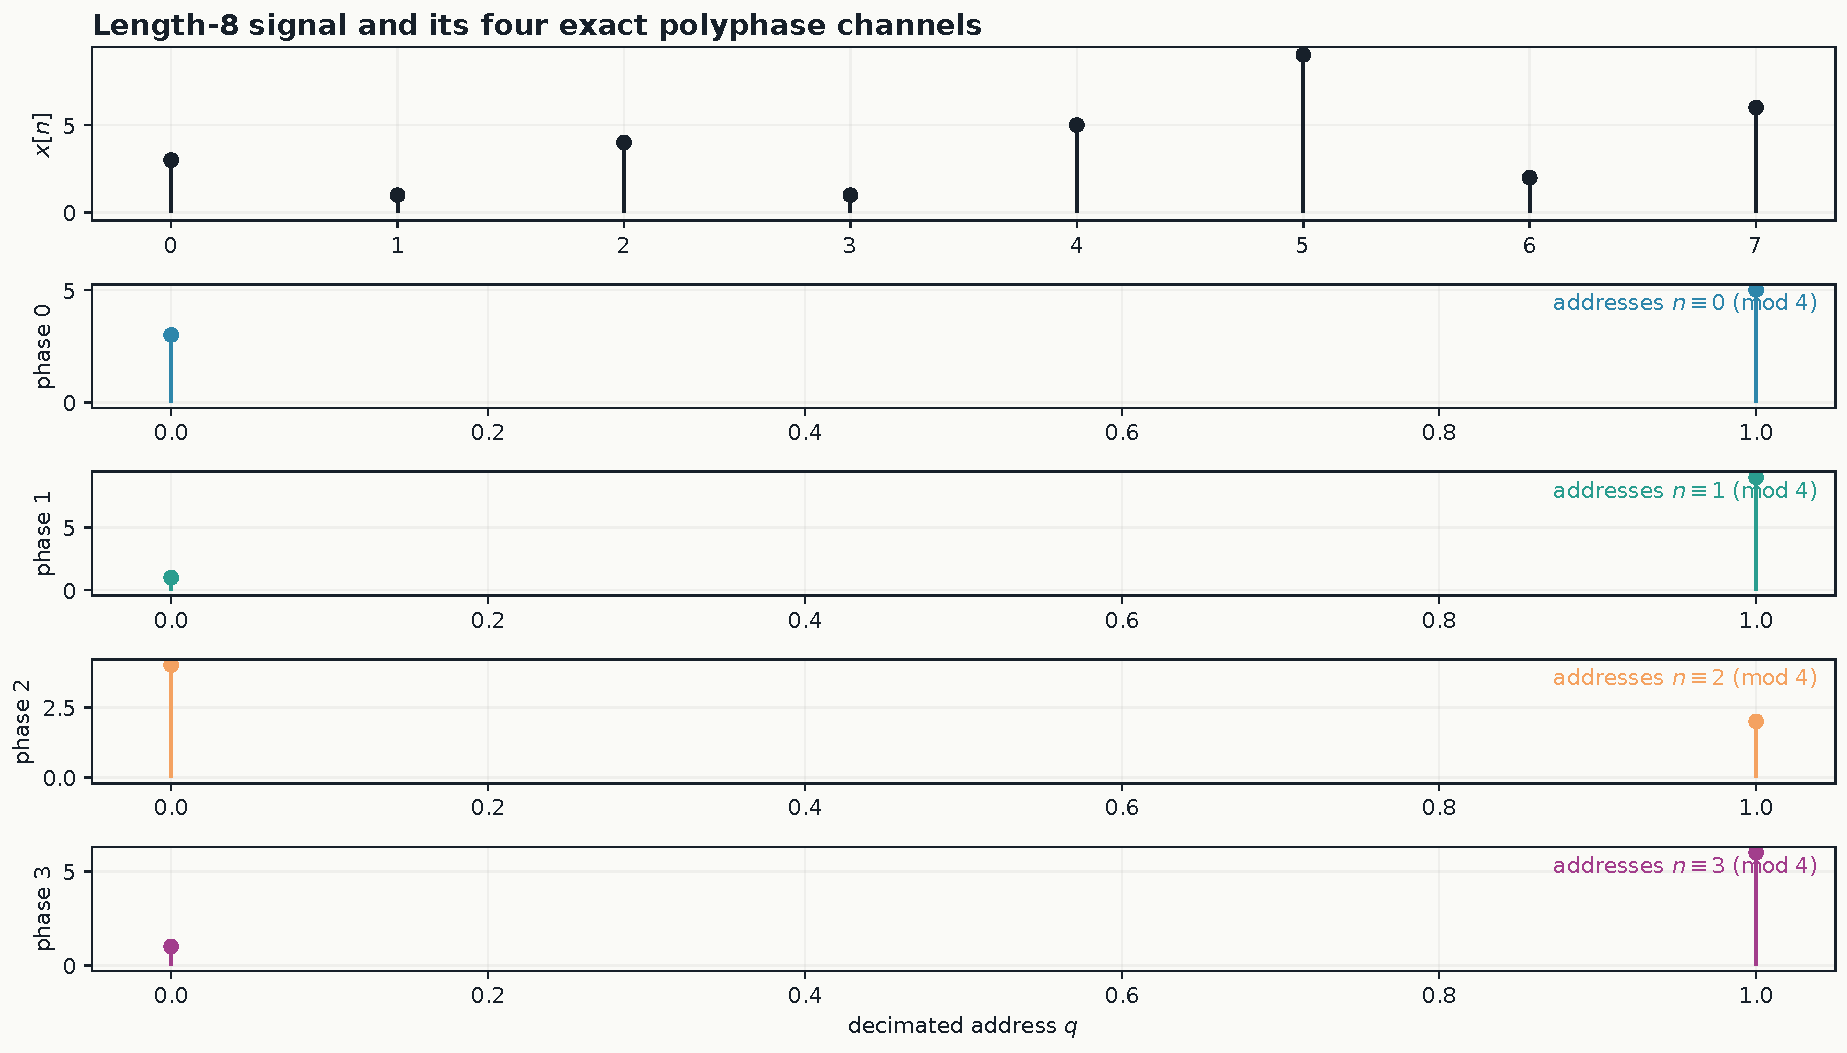
\includegraphics[width=.96\linewidth]{03_signal_polyphase.pdf}
\caption{The signal and its four exact phase channels. Each sample appears in one and only one packet.}
\end{figure}

\section{Step 3: nested phase refinement}
The order-two packets split as
\[
\boxed{P_{2,0}=P_{4,0}+P_{4,2}},
\qquad
\boxed{P_{2,1}=P_{4,1}+P_{4,3}}.
\]
At the channel level,
\[
(3,4,5,2)\longleftrightarrow (3,5)\oplus(4,2),
\]
and
\[
(1,1,9,6)\longleftrightarrow (1,9)\oplus(1,6).
\]
No interpolation is involved: refinement is address separation.

\section{Step 4: Haar analysis}
On every adjacent pair, use
\[
H_2=\frac1{\sqrt2}
\begin{pmatrix}1&1\\1&-1\end{pmatrix}.
\]
The block-diagonal one-level transform $H$ satisfies $H^{\mathsf T}H=I_8$. Its coefficients are
\[
Hx=
\left(
2\sqrt2,
\sqrt2,
\frac{5\sqrt2}{2},
\frac{3\sqrt2}{2},
7\sqrt2,
-2\sqrt2,
4\sqrt2,
-2\sqrt2
\right)^{\mathsf T}.
\]
Since $H^{-1}=H^{\mathsf T}$,
\[
\boxed{x=H^{\mathsf T}Hx.}
\]
This is the simplest orthonormal wavelet filter-bank realization of the transform-atlas theorem.

For each adjacent pair $(a,b)$, analysis produces
\[
\ell=\frac{a+b}{\sqrt2},
\qquad
h=\frac{a-b}{\sqrt2},
\]
and synthesis returns
\[
a=\frac{\ell+h}{\sqrt2},
\qquad
b=\frac{\ell-h}{\sqrt2}.
\]
For the first pair $(3,1)$ this gives $(\ell,h)=(2\sqrt2,\sqrt2)$ and then
\[
\frac{2\sqrt2+\sqrt2}{\sqrt2}=3,
\qquad
\frac{2\sqrt2-\sqrt2}{\sqrt2}=1.
\]
The same two-line inverse calculation reconstructs the other three pairs.

\SafeFigure[.98\linewidth]{23_signal_haar_butterfly.pdf}{The four Haar butterflies. Each box displays the exact low and detail coefficient generated from one adjacent sample pair.}{fig:haar-butterflies}

\section{Step 5: Fourier analysis as a projector atlas}
Let $F_8$ be the unitary discrete Fourier matrix,
\[
(F_8)_{jk}=\frac1{\sqrt8}e^{-2\pi ijk/8}.
\]
The coefficient vector is $\widehat x=F_8x$, and
\[
\boxed{x=F_8^*\widehat x.}
\]
Now group frequency coordinates into
\[
\{0\},\quad\{1,7\},\quad\{2,6\},\quad\{3,5\},\quad\{4\}.
\]
If $E_B$ selects one group, then
\[
Q_B=F_8^*E_BF_8
\]
is an exact projector in signal space. The five $Q_B$ are pairwise annihilating and sum to $I_8$.

The first and Nyquist coefficients are especially simple:
\[
\widehat x_0=\frac{31}{\sqrt8}=\frac{31\sqrt2}{4},
\qquad
\widehat x_4=-\frac3{\sqrt8}=-\frac{3\sqrt2}{4}.
\]
The conjugate symmetry $\widehat x_{8-k}=\overline{\widehat x_k}$ follows because $x$ is real.  The exact band energies are
\[
\begin{array}{c|c}
B&\norm{E_B\widehat x}_2^2\\
\hline
\{0\}&961/8\\
\{1,7\}&97/4-5\sqrt2\\
\{2,6\}&13/4\\
\{3,5\}&97/4+5\sqrt2\\
\{4\}&9/8
\end{array}
\]
and their sum is $173=\norm{x}_2^2$.

\SafeFigure[.98\linewidth]{24_signal_fourier_coefficients.pdf}{Magnitude and phase of all eight Fourier coefficients, together with the numerical inverse-transform residual. Both magnitude and phase are required for reconstruction.}{fig:fourier-coordinates}

\begin{figure}[H]
\centering
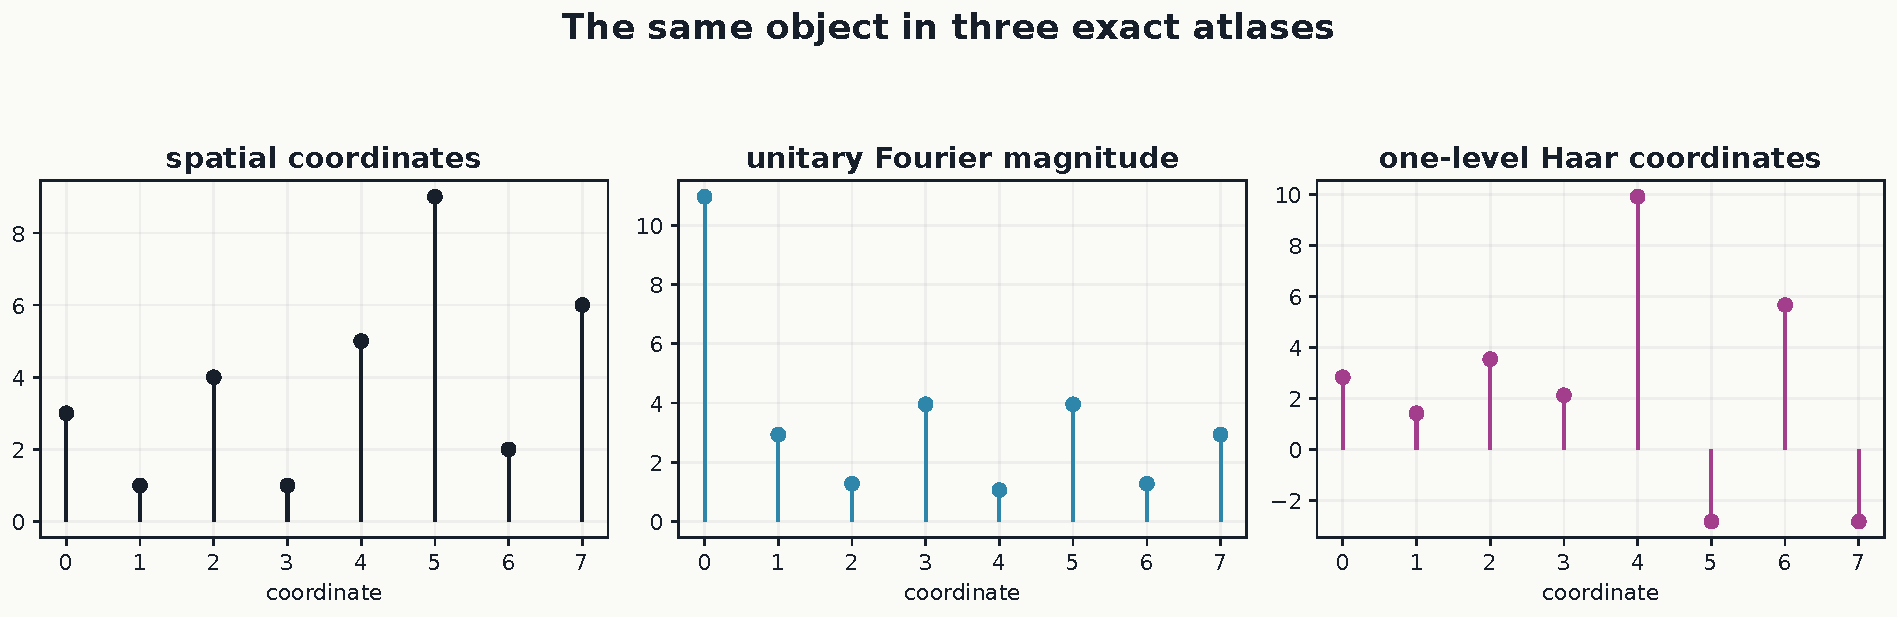
\includegraphics[width=.96\linewidth]{04_signal_three_atlases.pdf}
\caption{The same signal in spatial, Fourier, and Haar coordinates. Complete coordinates in each atlas reconstruct the same object.}
\end{figure}

\begin{figure}[H]
\centering
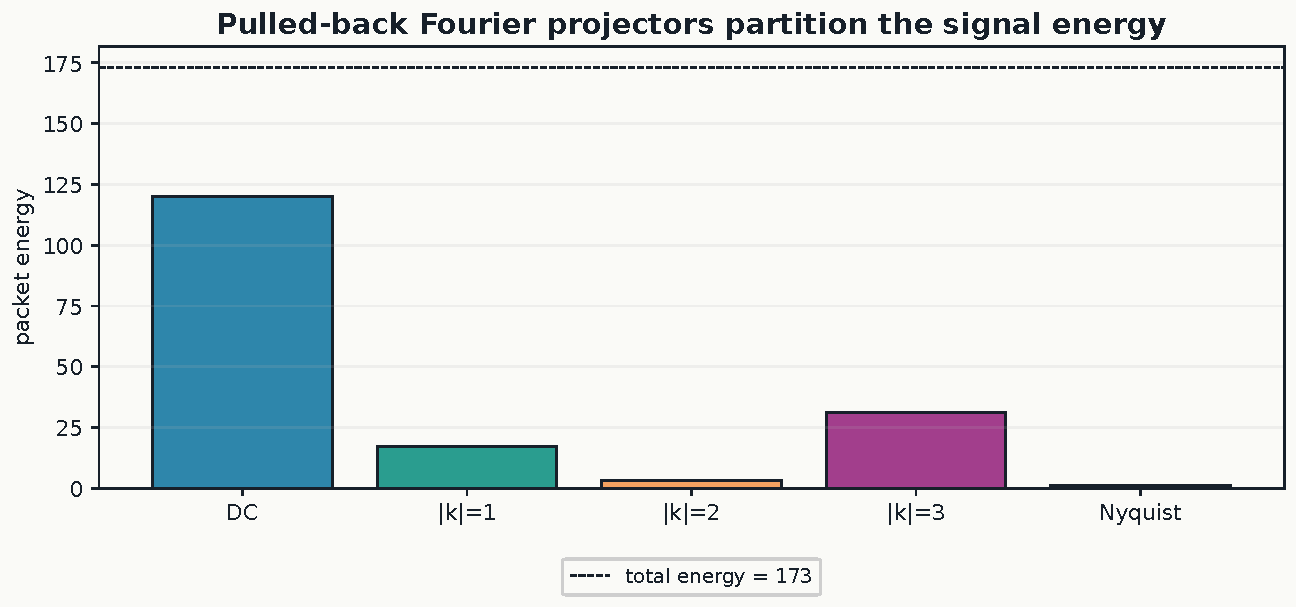
\includegraphics[width=.76\linewidth]{05_fourier_packet_energy.pdf}
\caption{The pulled-back Fourier packets partition the squared norm of the signal. The legend is placed below the plot so no data are obscured.}
\end{figure}

\SafeFigure[.96\linewidth]{25_signal_fourier_band_packets.pdf}{Each frequency selector is pulled back to the original sample coordinates. The five displayed packet signals add pointwise to the original signal.}{fig:fourier-band-signals}

\begin{auditbox}[ for the transform portfolio]
The polyphase, Haar, and Fourier constructions are checked by different inverses:
\begin{itemize}
\item polyphase synthesis uses address interleaving;
\item Haar synthesis uses the transpose of an orthogonal block matrix;
\item Fourier synthesis uses the conjugate transpose of a unitary complex matrix.
\end{itemize}
Agreement of all three reconstructions is therefore not one repeated implementation check. It is three algebraically distinct inverse calculations on the same object.
\end{auditbox}

\begin{certificate}
SymPy verifies exactly
\[
\begin{gathered}
\Scal_4\Acal_4x-x=0,\\
P_{2,0}-P_{4,0}-P_{4,2}=0,
\qquad
P_{2,1}-P_{4,1}-P_{4,3}=0,\\
H^{\mathsf T}H-I_8=0,
\qquad
H^{\mathsf T}Hx-x=0,\\
F_8^*F_8-I_8=0,
\qquad
F_8^*F_8x-x=0,\\
\sum_BQ_B-I_8=0,
\qquad
Q_B^2-Q_B=0\text{ for every band }B.
\end{gathered}
\]
The signal energy is
\[
\norm{x}_2^2=3^2+1^2+4^2+1^2+5^2+9^2+2^2+6^2=173.
\]
\end{certificate}

\section{Selected symbolic implementation}
\begin{lstlisting}
phase4 = polyphase_analyze(x, 4)
polyphase_residual = polyphase_synthesize(phase4, 8) - x

H = haar_one_level_matrix(8)
haar_residual = simplify(H.T * H * x - x)

F = dft8_matrix()
fourier_residual = simplify(F.conjugate().T * F * x - x)
Q = transform_projectors(F, ((0,), (1,7), (2,6), (3,5), (4,)))
\end{lstlisting}

\chapter{Area III: a quantum circuit as packet paths}\label{ch:quantum}

\section{Problem}
Prepare a Bell state from one seed, decompose the circuit into parity packet paths, reconstruct the state, and certify entanglement by an exact reduced density matrix.

\section{Step 1: Hilbert space and parity packets}
Use the computational basis
\[
|00\rangle,|01\rangle,|10\rangle,|11\rangle
\]
of $\C^2\otimes\C^2$. Define
\[
P_{\mathrm e}=|00\rangle\langle00|+|11\rangle\langle11|,
\]
\[
P_{\mathrm o}=|01\rangle\langle01|+|10\rangle\langle10|.
\]
Then
\[
P_{\mathrm e}+P_{\mathrm o}=I_4,
\qquad
P_{\mathrm e}P_{\mathrm o}=0.
\]

\section{Step 2: the circuit}
Begin with
\[
\psi_0=|00\rangle.
\]
Apply a Hadamard gate to the first qubit:
\[
\psi_1=(H\otimes I)|00\rangle
=\frac{|00\rangle+|10\rangle}{\sqrt2}.
\]
Apply CNOT:
\[
\psi_2=\operatorname{CNOT}\,\psi_1
=\frac{|00\rangle+|11\rangle}{\sqrt2}
=:|\Phi^+\rangle.
\]

In the ordered computational basis, the two circuit matrices are
\[
H\otimes I=\frac1{\sqrt2}
\begin{pmatrix}
1&0&1&0\\
0&1&0&1\\
1&0&-1&0\\
0&1&0&-1
\end{pmatrix},
\qquad
\operatorname{CNOT}=
\begin{pmatrix}
1&0&0&0\\
0&1&0&0\\
0&0&0&1\\
0&0&1&0
\end{pmatrix}.
\]
Multiplying by the seed vector gives
\[
\begin{pmatrix}1\\0\\0\\0\end{pmatrix}
\xmapsto{H\otimes I}
\frac1{\sqrt2}
\begin{pmatrix}1\\0\\1\\0\end{pmatrix}
\xmapsto{\operatorname{CNOT}}
\frac1{\sqrt2}
\begin{pmatrix}1\\0\\0\\1\end{pmatrix}.
\]

\SafeFigure[.96\linewidth]{26_quantum_state_evolution.pdf}{Computational-basis probabilities at the seed, intermediate, and final circuit stages. The Hadamard creates two branches; CNOT moves the odd intermediate branch into the even output packet.}{fig:quantum-evolution}

\section{Step 3: packet path expansion}
The intermediate state has one even and one odd contribution. The only nonzero paths are
\[
P_{\mathrm e}\operatorname{CNOT}P_{\mathrm e}(H\otimes I)P_{\mathrm e}|00\rangle
=\frac{|00\rangle}{\sqrt2},
\]
and
\[
P_{\mathrm e}\operatorname{CNOT}P_{\mathrm o}(H\otimes I)P_{\mathrm e}|00\rangle
=\frac{|11\rangle}{\sqrt2}.
\]
Their sum is $|\Phi^+\rangle$. Every output-odd path vanishes.

All four parity routes can be listed explicitly:
\[
\begin{array}{c|c|c}
\text{intermediate parity}&\text{output parity}&\text{path vector}\\
\hline
e&e&(1,0,0,0)^{\mathsf T}/\sqrt2\\
o&e&(0,0,0,1)^{\mathsf T}/\sqrt2\\
e&o&0\\
o&o&0
\end{array}
\]
The path sum is coherent: vectors are added before probabilities are formed.  In this example the two surviving outputs are orthogonal basis states, so the final computational-basis probabilities are $1/2$ at $00$ and $1/2$ at $11$.

\SafeFigure[.92\linewidth]{27_quantum_path_and_measurement.pdf}{Left: squared norms of all four parity paths. Right: the final measurement distribution. The two zero paths are shown rather than omitted.}{fig:quantum-path-table}

\begin{figure}[H]
\centering
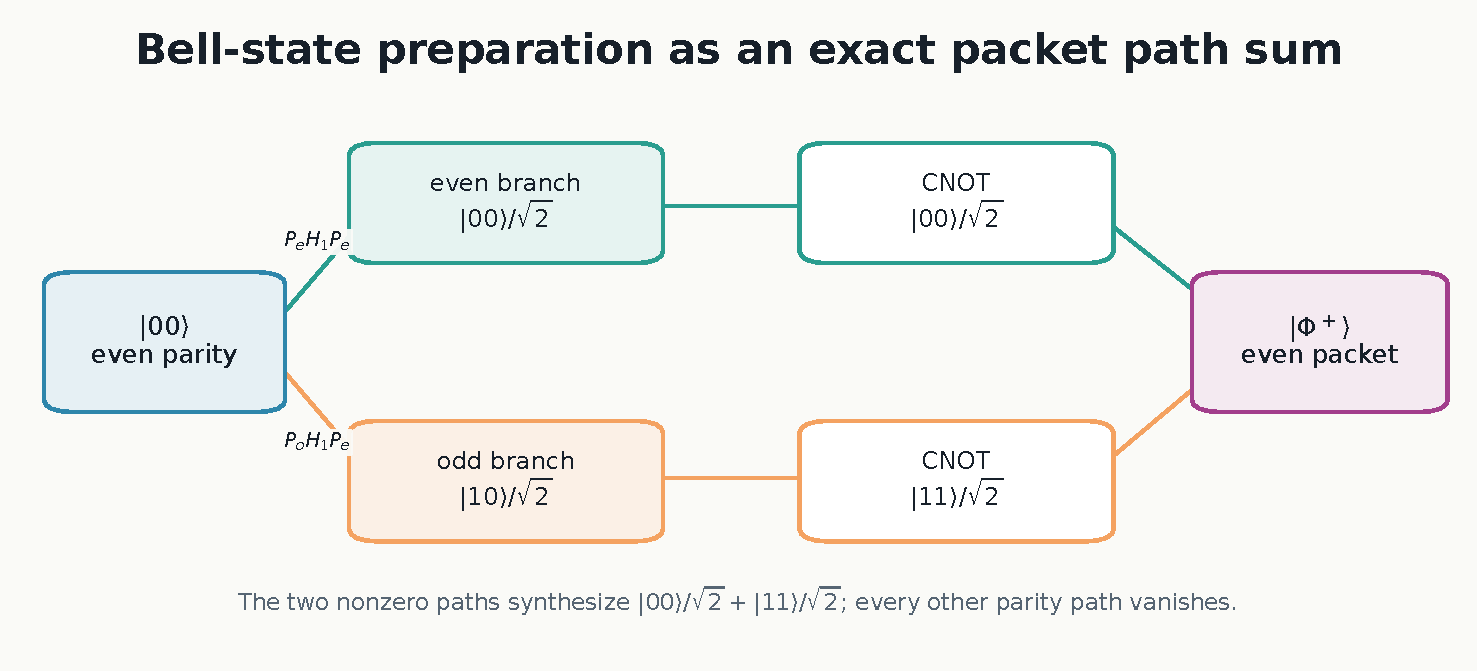
\includegraphics[width=.96\linewidth]{06_quantum_packet_paths.pdf}
\caption{The Bell circuit resolved into the two nonzero parity paths.}
\end{figure}

\section{Step 4: density matrix and partial trace}
The pure-state density matrix is
\[
\rho=|\Phi^+\rangle\langle\Phi^+|
=\frac12
\begin{pmatrix}
1&0&0&1\\
0&0&0&0\\
0&0&0&0\\
1&0&0&1
\end{pmatrix}.
\]
Tracing out the second qubit gives
\[
\rho_A=\Tr_B(\rho)=\frac12I_2.
\]
Hence the first qubit is maximally mixed even though the two-qubit state is pure. This is an exact entanglement certificate.

The eigenvalues of $\rho_A$ are $(1/2,1/2)$, so its von Neumann entropy is
\[
S(\rho_A)=-\Tr(\rho_A\log_2\rho_A)
=-2\left(\frac12\log_2\frac12\right)=1.
\]
A pure bipartite state with a mixed reduced state cannot factor as $|u\rangle\otimes|v\rangle$.  Thus the partial-trace calculation certifies one full ebit of entanglement.

\begin{figure}[H]
\centering
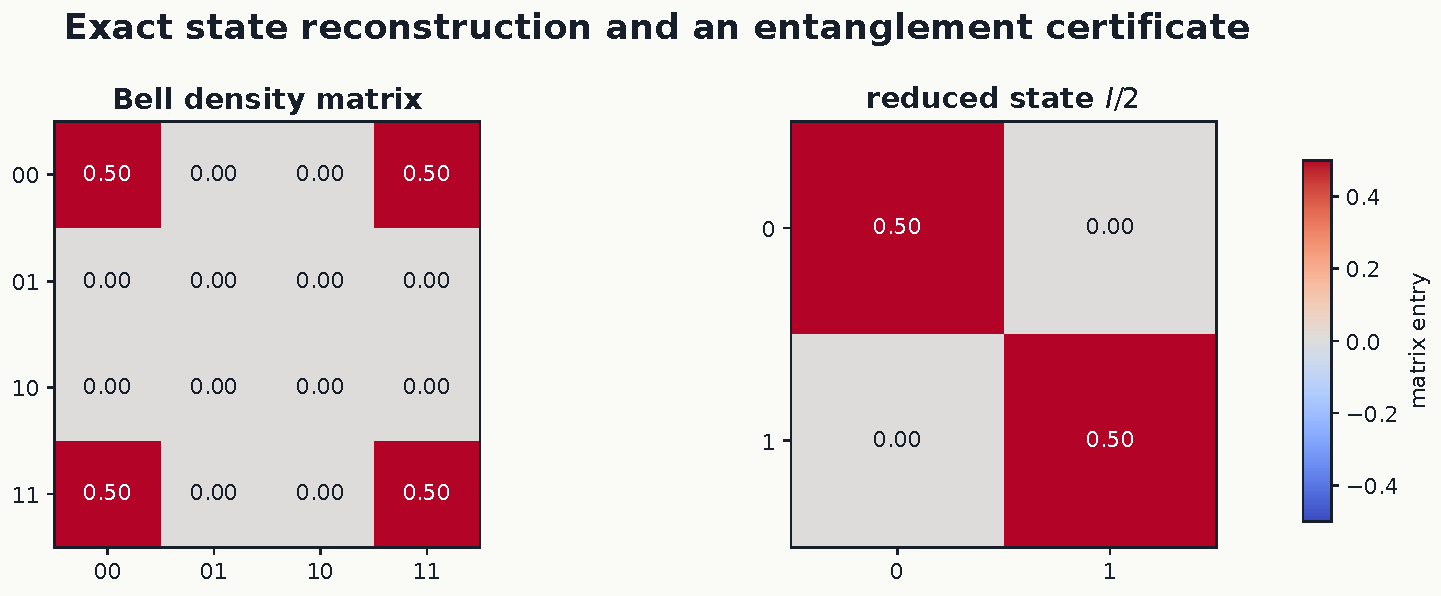
\includegraphics[width=.82\linewidth]{07_quantum_density.pdf}
\caption{The Bell density matrix and its reduced one-qubit state.}
\end{figure}

\begin{certificate}
The symbolic computation returns
\[
\begin{aligned}
&\norm{\psi_2}^2-1=0,\\
&P_{\mathrm o}\psi_2=0,\\
&\left(P_{\mathrm e}\operatorname{CNOT}P_{\mathrm e}H_1P_{\mathrm e}
+P_{\mathrm e}\operatorname{CNOT}P_{\mathrm o}H_1P_{\mathrm e}\right)|00\rangle-\psi_2=0,\\
&\Tr_B(\rho)-\frac12I_2=0.
\end{aligned}
\]
\end{certificate}

\section{Selected symbolic implementation}
\begin{lstlisting}
psi1 = (H \otimes I2) * psi0
bell = CNOT * psi1

path_even = Pe * CNOT * Pe * H1 * Pe * psi0
path_odd  = Pe * CNOT * Po * H1 * Pe * psi0
path_residual = path_even + path_odd - bell

rho = bell * bell.conjugate().T
rho_A = partial_trace_second_qubit(rho)
\end{lstlisting}

\chapter{Area IV: stochastic projectors and Bayesian refinement}\label{ch:bayes}

\section{Problem}
Show that conditional expectation is an exact projector, prove when Bayesian conditioning commutes with packet coarsening, and factor the failure exactly when the likelihood varies inside a packet.

\section{Step 1: a conditional-expectation projector}
Use the finite probability measure
\[
\mu=\left(\frac1{10},\frac2{10},\frac3{10},\frac4{10}\right)
\]
and the partition
\[
A=\{0,1\},\qquad B=\{2,3\}.
\]
Conditional expectation onto packet-constant observables is represented by
\[
E_\pi=
\begin{pmatrix}
\frac13&\frac23&0&0\\
\frac13&\frac23&0&0\\
0&0&\frac37&\frac47\\
0&0&\frac37&\frac47
\end{pmatrix}.
\]
For
\[
f=(1,4,-2,3)^{\mathsf T},
\]
we obtain
\[
E_\pi f=\left(3,3,\frac67,\frac67\right)^{\mathsf T}.
\]
Direct multiplication proves
\[
E_\pi^2=E_\pi.
\]
If $M=\diag(\mu)$, then
\[
ME_\pi=E_\pi^{\mathsf T}M,
\]
so $E_\pi$ is self-adjoint for the weighted inner product $\ip{u}{v}_\mu=u^{\mathsf T}Mv$.

The residual is
\[
r=f-E_\pi f=
\left(-2,1,-\frac{20}{7},\frac{15}{7}\right)^{\mathsf T}.
\]
Let $\mathbf1_A=(1,1,0,0)^{\mathsf T}$ and $\mathbf1_B=(0,0,1,1)^{\mathsf T}$.  Direct calculation gives
\[
\ip{r}{\mathbf1_A}_\mu
=\frac1{10}(-2)+\frac2{10}(1)=0,
\]
\[
\ip{r}{\mathbf1_B}_\mu
=\frac3{10}\left(-\frac{20}{7}\right)
+\frac4{10}\left(\frac{15}{7}\right)=0.
\]
Since packet-constant observables are spanned by $\mathbf1_A$ and $\mathbf1_B$, the residual is orthogonal to the entire target subspace.

\SafeFigure[.96\linewidth]{28_bayes_weighted_projection.pdf}{The observable, its conditional expectation, and the residual. The right panel displays the two weighted inner products that vanish exactly.}{fig:bayes-weighted-orthogonality}

\begin{figure}[H]
\centering
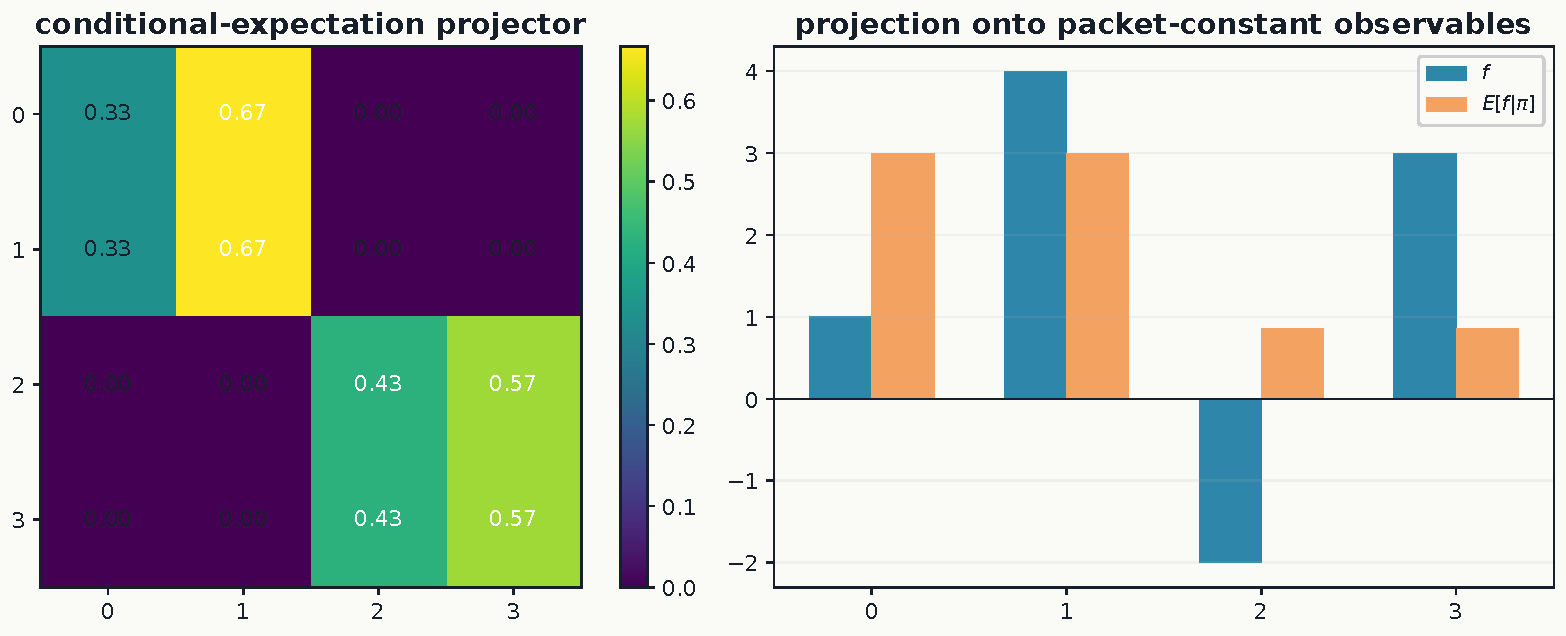
\includegraphics[width=.91\linewidth]{08_conditional_expectation.pdf}
\caption{The finite conditional-expectation projector and its action on one observable.}
\end{figure}

\section{Step 2: Bayesian conditioning}
For prior $p$ and positive likelihood $\lambda$, define
\[
\Bcal_\lambda(p)_i
=\frac{\lambda_i p_i}{\sum_j\lambda_jp_j}.
\]
Let $C_\pi p=(P_A,P_B)$ denote coarse packet masses.

\begin{theorem}[Exact effective coarse likelihood]\label{thm:effective-likelihood}
For every prior with positive packet masses, define
\[
r_a(p)=\frac{\sum_{i\in I_a}\lambda_ip_i}{P_a}.
\]
Then
\[
\boxed{C_\pi\Bcal_\lambda(p)=\Bcal_{r(p)}(C_\pi p).}
\]
\end{theorem}

\begin{proof}
The $a$th coarse posterior mass is
\[
\sum_{i\in I_a}\frac{\lambda_ip_i}{\sum_j\lambda_jp_j}
=\frac{P_ar_a(p)}{\sum_bP_br_b(p)},
\]
which is exactly the coarse Bayesian update with likelihood $r(p)$.
\end{proof}

\begin{theorem}[Finite sufficiency criterion]
Assume at least two coarse packets can carry positive prior mass.  A fixed coarse likelihood $\bar\lambda$ satisfies
\[
C_\pi\Bcal_\lambda(p)=\Bcal_{\bar\lambda}(C_\pi p)
\]
for every strictly positive fine prior $p$ if and only if there is one scalar $c>0$ such that
\[
\lambda_i=c\,\bar\lambda_a
\qquad(i\in I_a).
\]
Equivalently, after removal of one globally invisible scale, the likelihood must be constant inside every packet.
\end{theorem}

\begin{proof}
The stated condition is sufficient because then $r_a(p)=c\bar\lambda_a$ for every prior, and the common scale cancels in Bayesian normalization.  Conversely, fix the coarse packet masses and vary the conditional distribution inside one packet.  If two fine likelihood values in that packet differ, its weighted average $r_a(p)$ changes while the coarse prior stays fixed.  Placing positive mass on another packet makes this change visible after normalization, contradicting prior-independent coarse closure.
\end{proof}

\section{Step 3: the sufficient case}
Take
\[
\lambda=(2,2,1,1)^{\mathsf T}.
\]
The likelihood is constant inside each packet, so $r=(2,1)$ independently of the hidden fine prior. The fine posterior is
\[
\Bcal_\lambda(\mu)
=\left(\frac2{13},\frac4{13},\frac3{13},\frac4{13}\right)^{\mathsf T}.
\]
Coarsening gives
\[
\left(\frac6{13},\frac7{13}\right)^{\mathsf T},
\]
which agrees exactly with the coarse update of $(3/10,7/10)$ by likelihood $(2,1)$.

\section{Step 4: the nonsufficient case}
Now take
\[
\lambda=(1,3,2,4)^{\mathsf T}.
\]
The effective packet likelihoods are
\[
r_A=\frac73,
\qquad
r_B=\frac{22}{7}.
\]
Therefore the exact coarse posterior is
\[
C_\pi\Bcal_\lambda(\mu)
=\left(\frac7{29},\frac{22}{29}\right)^{\mathsf T}.
\]
If one incorrectly replaces the hidden likelihood structure by the nominal coarse likelihood
\[
\bar\lambda=(2,3)^{\mathsf T},
\]
then the nominal posterior is
\[
\Bcal_{\bar\lambda}(C_\pi\mu)
=\left(\frac29,\frac79\right)^{\mathsf T}.
\]
The defect is
\[
\boxed{
\left(\frac7{29},\frac{22}{29}\right)
-
\left(\frac29,\frac79\right)
=
\left(\frac5{261},-\frac5{261}\right).
}
\]

The necessity of the sufficiency criterion can also be seen with two priors having exactly the same coarse packet masses:
\[
p^{(1)}=\left(\frac1{10},\frac2{10},\frac3{10},\frac4{10}\right),
\qquad
p^{(2)}=\left(\frac2{10},\frac1{10},\frac4{10},\frac3{10}\right).
\]
Both coarsen to $(3/10,7/10)$, but the same fine likelihood $(1,3,2,4)$ produces
\[
C_\pi\Bcal_\lambda(p^{(1)})=\left(\frac7{29},\frac{22}{29}\right),
\qquad
C_\pi\Bcal_\lambda(p^{(2)})=\left(\frac15,\frac45\right).
\]
Their difference is
\[
\left(\frac6{145},-\frac6{145}\right)\ne0.
\]
Therefore the coarse prior alone cannot determine the coarse posterior when within-packet likelihoods differ.

\SafeFigure[.98\linewidth]{29_bayes_same_coarse_witness.pdf}{Two different fine priors have the same coarse masses but produce different coarse posteriors. This is a direct finite witness of information loss under nonsufficient coarsening.}{fig:bayes-prior-witness}

\begin{figure}[H]
\centering
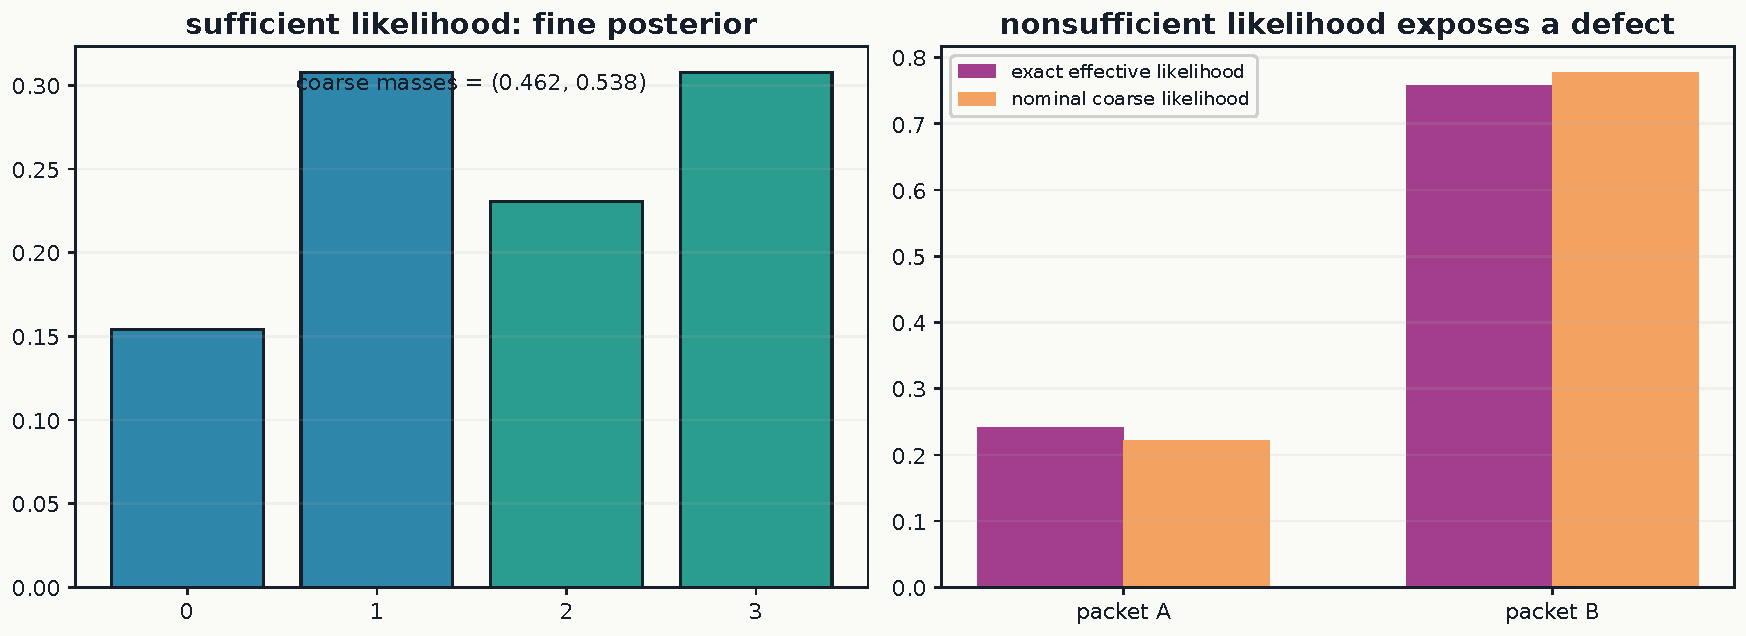
\includegraphics[width=.94\linewidth]{09_bayesian_updates.pdf}
\caption{Sufficient packet conditioning and a nonsufficient negative control.}
\end{figure}

\section{Step 5: exact information-loss factorization}
Let
\[
P=C_\pi p,
\qquad
\delta=r(p)-\bar\lambda,
\qquad
\bar b=\Bcal_{\bar\lambda}(P),
\qquad
Z_r=\ip{r(p)}{P}.
\]
Then direct algebra gives
\[
\boxed{
C_\pi\Bcal_\lambda(p)-\Bcal_{\bar\lambda}(P)
=
\frac1{Z_r}
\left(\diag(P)-\bar bP^{\mathsf T}\right)\delta.
}
\]
The defect is therefore carried entirely by the within-packet likelihood variation $\delta$.

For the numerical example,
\[
P=\begin{pmatrix}3/10\\7/10\end{pmatrix},
\quad
r=\begin{pmatrix}7/3\\22/7\end{pmatrix},
\quad
\bar\lambda=\begin{pmatrix}2\\3\end{pmatrix},
\quad
\delta=\begin{pmatrix}1/3\\1/7\end{pmatrix},
\]
\[
Z_r=P^{\mathsf T}r=\frac{29}{10},
\qquad
\bar b=\begin{pmatrix}2/9\\7/9\end{pmatrix},
\]
and
\[
\diag(P)-\bar bP^{\mathsf T}
=
\begin{pmatrix}
7/30&-7/45\\
-7/30&7/45
\end{pmatrix}.
\]
Multiplication gives
\[
\frac{1}{Z_r}
\left(\diag(P)-\bar bP^{\mathsf T}\right)\delta
=
\begin{pmatrix}5/261\\-5/261\end{pmatrix},
\]
exactly matching the directly computed defect.

\begin{proof}
Write $r=\bar\lambda+\delta$. Since
\[
\Bcal_r(P)=\frac{\diag(P)r}{Z_r},
\]
and
\[
\bar b=\frac{\diag(P)\bar\lambda}{Z_{\bar\lambda}},
\]
subtract the two fractions, replace $Z_r-Z_{\bar\lambda}$ by $P^{\mathsf T}\delta$, and collect the $\delta$ terms. The displayed factorization follows.
\end{proof}

\begin{figure}[H]
\centering
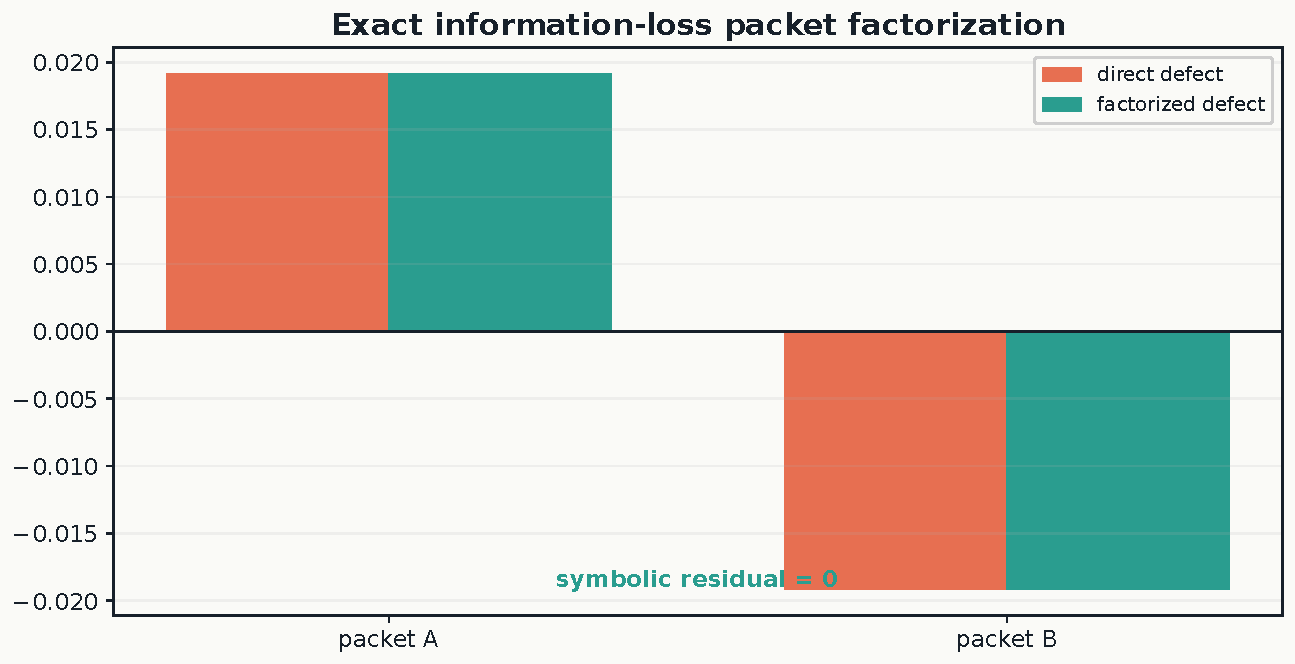
\includegraphics[width=.74\linewidth]{10_bayesian_defect_factorization.pdf}
\caption{The direct Bayesian defect and the factorized information-loss packet agree exactly.}
\end{figure}

\begin{certificate}
The exact residuals are
\[
E_\pi^2-E_\pi=0,
\qquad
ME_\pi-E_\pi^{\mathsf T}M=0,
\]
\[
C_\pi\Bcal_{(2,2,1,1)}(\mu)
-\Bcal_{(2,1)}(C_\pi\mu)=0,
\]
and
\[
\left[C_\pi\Bcal_\lambda(\mu)-\Bcal_{\bar\lambda}(C_\pi\mu)\right]
-
\frac{\diag(P)-\bar bP^{\mathsf T}}{Z_r}\delta
=0.
\]
\end{certificate}

\chapter{Area V: a closed root-filter family and a candidate integer sequence}\label{ch:arithmetic}

\section{Problem}
Generate an exact integer sequence from a projector-resolved analytic seed, derive its root-sum and hypergeometric closed forms, prove an integer recurrence, prove a second finite composition formula, and produce a candidate OEIS record.

\section{Step 1: the signed order-five packet}
Define
\[
D_5(z)=\sum_{n\ge0}(-1)^n\frac{z^{5n}}{(5n)!}.
\]
This is the residue-zero packet of an exponential system whose fifth derivative returns the negative of the original function:
\[
D_5^{(5)}=-D_5.
\]

Let
\[
\eta_k=\exp\!\left(\frac{(2k+1)\pi i}{5}\right),
\qquad 0\le k<5,
\]
so that $\eta_k^5=-1$.  The root filter gives
\[
\boxed{D_5(z)=\frac15\sum_{k=0}^{4}e^{\eta_k z}.}
\]
Indeed,
\[
\frac15\sum_{k=0}^{4}e^{\eta_kz}
=
\sum_{m\ge0}
\left(\frac15\sum_{k=0}^{4}\eta_k^m\right)
\frac{z^m}{m!}.
\]
The inner sum vanishes unless $5\mid m$.  For $m=5n$ it equals
\[
\frac15\sum_{k=0}^{4}(\eta_k^5)^n=(-1)^n,
\]
which selects exactly the coefficients of $D_5$.

\SafeFigure[.72\linewidth]{30_arithmetic_signed_roots.pdf}{The five roots of $\eta^5=-1$. Their character average annihilates every exponential coefficient outside degrees divisible by five.}{fig:signed-five-roots}

Pairing conjugate roots yields the real closed form
\[
\boxed{
\begin{aligned}
D_5(z)=\frac15\Bigg[&e^{-z}
+2e^{az}\cos(bz)
+2e^{cz}\cos(dz)\Bigg],
\end{aligned}}
\]
where
\[
a=\frac{1+\sqrt5}{4},
\quad
b=\frac{\sqrt{10-2\sqrt5}}4,
\quad
c=\frac{1-\sqrt5}{4},
\quad
d=\frac{\sqrt{10+2\sqrt5}}4.
\]

The factorial multiplication formula also gives
\[
\boxed{
D_5(z)
={}_0F_4\!\left(
\begin{matrix}-\\[1pt]\frac15,\frac25,\frac35,\frac45\end{matrix};
-\frac{z^5}{5^5}
\right).
}
\]
To verify this term by term, use
\[
(5n)!=5^{5n}n!
\left(\frac15\right)_n
\left(\frac25\right)_n
\left(\frac35\right)_n
\left(\frac45\right)_n.
\]
The $n$th hypergeometric term is therefore exactly $(-1)^nz^{5n}/(5n)!$.

\section{Step 2: reciprocal square and sequence definition}
Define
\[
S(z)=D_5(z)^{-2}
=\sum_{n\ge0}a_n\frac{z^{5n}}{(5n)!}.
\]
Using the closed form for $D_5$,
\[
\boxed{
S(z)=
\frac{25}{\left[e^{-z}+2e^{az}\cos(bz)+2e^{cz}\cos(dz)\right]^2}.
}
\]
This is a genuine closed analytic formula for the whole sequence-generating function.

\begin{figure}[H]
\centering
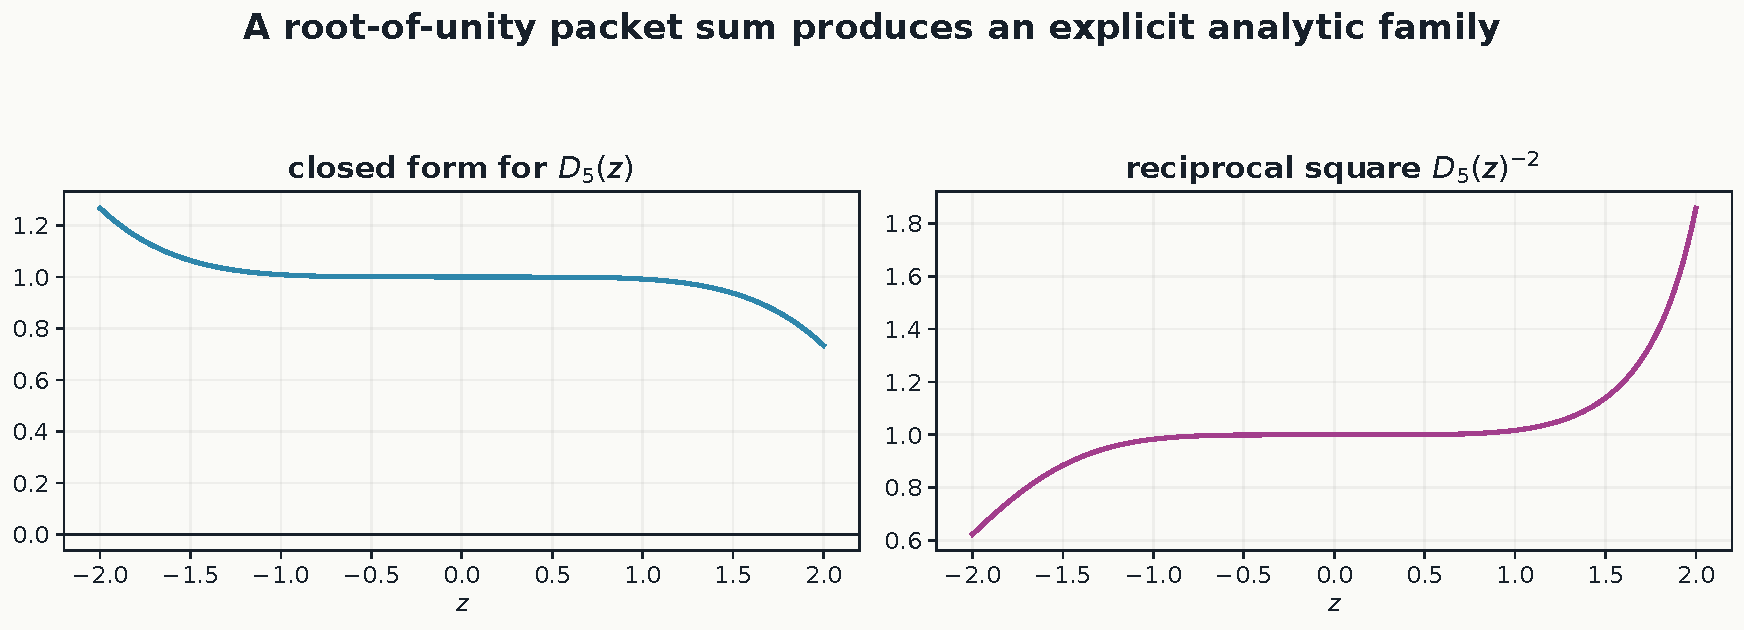
\includegraphics[width=.92\linewidth]{12_candidate_sequence_closed_form.pdf}
\caption{The signed root-filter denominator and its reciprocal square.}
\end{figure}

\section{Step 3: an exact integer recurrence}
Logarithmic differentiation of $S=D_5^{-2}$ gives
\[
D_5S'+2D_5'S=0.
\]
Extracting the coefficient of $z^{5n-1}/(5n-1)!$ gives, for $n\ge1$,
\[
\boxed{
\begin{aligned}
a_n={}&-
\sum_{k=1}^{n-1}(-1)^k
\binom{5n-1}{5k}a_{n-k}\\
&-2\sum_{k=1}^{n}(-1)^k
\binom{5n-1}{5k-1}a_{n-k},
\qquad a_0=1.
\end{aligned}}
\]
Every coefficient on the right is an integer. Induction proves
\[
\boxed{a_n\in\mathbb Z\quad(n\ge0).}
\]

The first four nontrivial rows show how the recurrence works:
\[
\begin{array}{c|r|r|r}
n&\text{first convolution contribution}&\text{derivative contribution}&a_n\\
\hline
1&0&2&2\\
2&252&502&754\\
3&1{,}507{,}506&1{,}501{,}502&3{,}009{,}008\\
4&34{,}919{,}099{,}764&23{,}186{,}570{,}502&58{,}105{,}670{,}266
\end{array}
\]
Each row is an exact integer identity, not a rounded numerical evaluation.

\SafeFigure[.90\linewidth]{31_arithmetic_recurrence_contributions.pdf}{The two integral contributions to the first four nontrivial recurrence rows. Heights are normalized by the exact total so that both contributions remain visible; exact integers are printed inside the bars.}{fig:arithmetic-recurrence-contributions}

The first terms are
\[
\begin{aligned}
1,&\ 2,\ 754,\ 3009008,\ 58105670266,\ 3690819041733782,\\
&611297487195595912564,\\
&225925381294863591587930378,\\
&166595785020134064487394817914506,\ldots
\end{aligned}
\]

\begin{figure}[H]
\centering
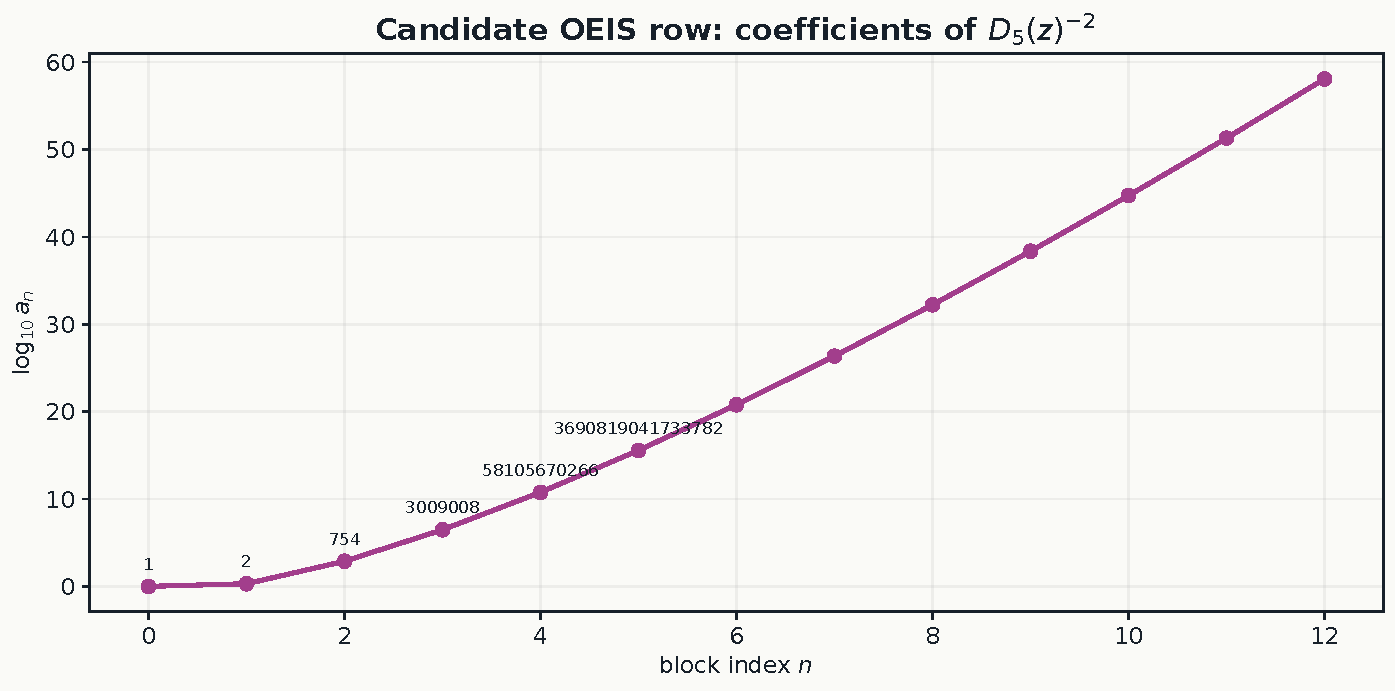
\includegraphics[width=.78\linewidth]{11_candidate_sequence_growth.pdf}
\caption{Growth of the candidate sequence on a base-ten logarithmic scale. Only the first few terms are annotated to prevent label collisions.}
\end{figure}

\SafeFigure[.92\linewidth]{32_arithmetic_digit_growth.pdf}{Two readable summaries of the same rapid growth: decimal digit count and base-ten logarithm.}{fig:arithmetic-digit-growth}

\section{Step 4: an independent finite coefficient formula}
Write
\[
D_5(z)=1+u(z),
\qquad
u(z)=\sum_{k\ge1}(-1)^k\frac{z^{5k}}{(5k)!}.
\]
Since
\[
(1+u)^{-2}=\sum_{m\ge0}(-1)^m(m+1)u^m,
\]
the coefficient is
\[
\boxed{
 a_n
 =(5n)!\sum_{m=1}^{n}(-1)^{n+m}(m+1)
 \sum_{\substack{k_1+\cdots+k_m=n\\k_i\ge1}}
 \prod_{i=1}^{m}\frac1{(5k_i)!}
}
\]
for $n\ge1$, with $a_0=1$.

This formula and the recurrence arise from different algebraic operations. Their exact agreement through the computed range is therefore an independent internal check.

\section{Step 5: the reciprocal-order polynomial family}
More generally, define
\[
D_5(z)^{-r}
=\sum_{n\ge0}P_{5,n}(r)\frac{z^{5n}}{(5n)!}.
\]
The first parameter polynomials are
\[
\begin{aligned}
P_{5,0}(r)&=1,\\
P_{5,1}(r)&=r,\\
P_{5,2}(r)&=r(126r+125),\\
P_{5,3}(r)&=r(126126r^2+375375r+249250),\\
P_{5,4}(r)&=r(488864376r^3+2909907000r^2\\
&\hspace{1.25in}+5307778250r+2886735625).
\end{aligned}
\]
They satisfy the semigroup convolution
\[
\boxed{
P_{5,n}(r+s)
=\sum_{q=0}^n\binom{5n}{5q}P_{5,q}(r)P_{5,n-q}(s).
}
\]
Our sequence is the row $a_n=P_{5,n}(2)$.

\begin{figure}[H]
\centering
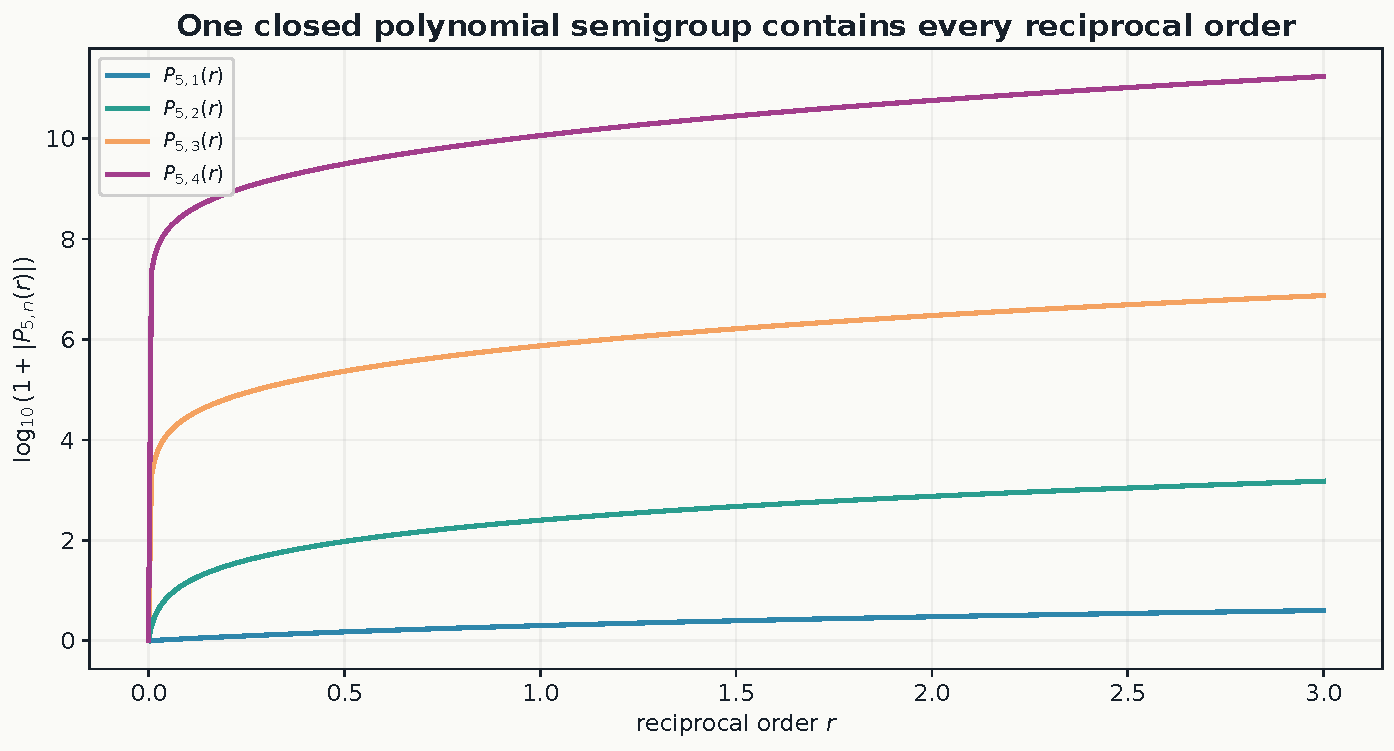
\includegraphics[width=.82\linewidth]{13_parameter_polynomials.pdf}
\caption{The first order-five reciprocal parameter polynomials.}
\end{figure}

\section{OEIS-style candidate record}
The sequence is supplied in an OEIS-ready form because its definition, recurrence, initial values, and b-file are exact.  This document does not assert historical novelty or the absence of an equivalent transformed sequence.  The mathematical claim proved here is narrower and complete:
\[
\boxed{
D_5(z)^{-2}
=\sum_{n\ge0}a_n\frac{z^{5n}}{(5n)!},
\qquad
(a_n)_{n\ge0}\subset\mathbb Z,
}
\]
with the displayed recurrence and independent composition formula.  Any database identifier would be metadata added after mathematical equivalence is established; it is not used in any proof.

\begin{certificate}
The symbolic package verifies:
\begin{enumerate}[label=(\roman*)]
\item every recurrence residual through $n=12$ is exactly zero;
\item multiplying the block series for $D_5^2$ by the candidate block series gives $1$ through the same exact range;
\item the hypergeometric coefficient identity is exact term by term;
\item the composition formula equals the recurrence values for every computed term;
\item every computed $a_n$ is an integer.
\end{enumerate}
\end{certificate}

\section{Selected symbolic implementation}
\begin{lstlisting}
def transfer_secancy_coefficients(N, r, nmax):
    vals = [Integer(1)]
    for n in range(1, nmax + 1):
        first = -sum((-1)**k * binomial(N*n-1, N*k)
                     * vals[n-k] for k in range(1, n))
        second = -r * sum((-1)**k * binomial(N*n-1, N*k-1)
                          * vals[n-k] for k in range(1, n+1))
        vals.append(factor(expand(first + second)))
    return vals
\end{lstlisting}

\chapter{Area VI: a coupled-oscillator physics problem}\label{ch:physics}

\section{Problem}
Solve a two-mass coupled oscillator exactly, identify its normal-mode projectors, reconstruct the motion from the packets, and prove conservation and partition of energy.

\section{Step 1: equations of motion}
With unit masses and fixed-end nearest-neighbor springs, use
\[
q''(t)+Kq(t)=0,
\qquad
K=\begin{pmatrix}2&-1\\-1&2\end{pmatrix}.
\]
The characteristic polynomial is
\[
\det(K-\lambda I)
=(2-\lambda)^2-1
=(\lambda-1)(\lambda-3).
\]
Normalized eigenvectors are
\[
e_s=\frac1{\sqrt2}\begin{pmatrix}1\\1\end{pmatrix},
\qquad
 e_a=\frac1{\sqrt2}\begin{pmatrix}1\\-1\end{pmatrix},
\]
with
\[
Ke_s=e_s,
\qquad
Ke_a=3e_a.
\]
The symmetric and antisymmetric projectors are therefore the rank-one spectral projectors
\[
P_s=e_se_s^{\mathsf T}
=\frac12\begin{pmatrix}1&1\\1&1\end{pmatrix},
\qquad
P_a=e_ae_a^{\mathsf T}
=\frac12\begin{pmatrix}1&-1\\-1&1\end{pmatrix}.
\]

\SafeFigure[.86\linewidth]{33_physics_mode_shapes.pdf}{The two normalized eigenmodes of the stiffness matrix. Equal signs indicate in-phase motion; opposite signs indicate out-of-phase motion.}{fig:physics-mode-shapes}
They satisfy
\[
P_sP_a=0,
\qquad
P_s+P_a=I_2.
\]
Moreover,
\[
\boxed{K=P_s+3P_a.}
\]
Thus the two packet frequencies are
\[
\omega_s=1,
\qquad
\omega_a=\sqrt3.
\]

\section{Step 2: exact modal solution}
For initial position $q_0$ and velocity $v_0$,
\[
\boxed{
\begin{aligned}
q(t)={}&\cos(t)P_sq_0+\sin(t)P_sv_0\\
&+\cos(\sqrt3t)P_aq_0
+\frac{\sin(\sqrt3t)}{\sqrt3}P_av_0.
\end{aligned}}
\]
Take
\[
q_0=(1,0)^{\mathsf T},
\qquad
v_0=(0,0)^{\mathsf T}.
\]
The initial displacement packets are
\[
P_sq_0=\frac12\begin{pmatrix}1\\1\end{pmatrix},
\qquad
P_aq_0=\frac12\begin{pmatrix}1\\-1\end{pmatrix}.
\]
Thus half of the coordinate amplitude is initially in each mode, but the mode energies differ because the antisymmetric stiffness eigenvalue is three times larger.

Then
\[
\boxed{
q_1(t)=\frac{\cos t+\cos(\sqrt3t)}2,
\qquad
q_2(t)=\frac{\cos t-\cos(\sqrt3t)}2.
}
\]

\begin{figure}[H]
\centering
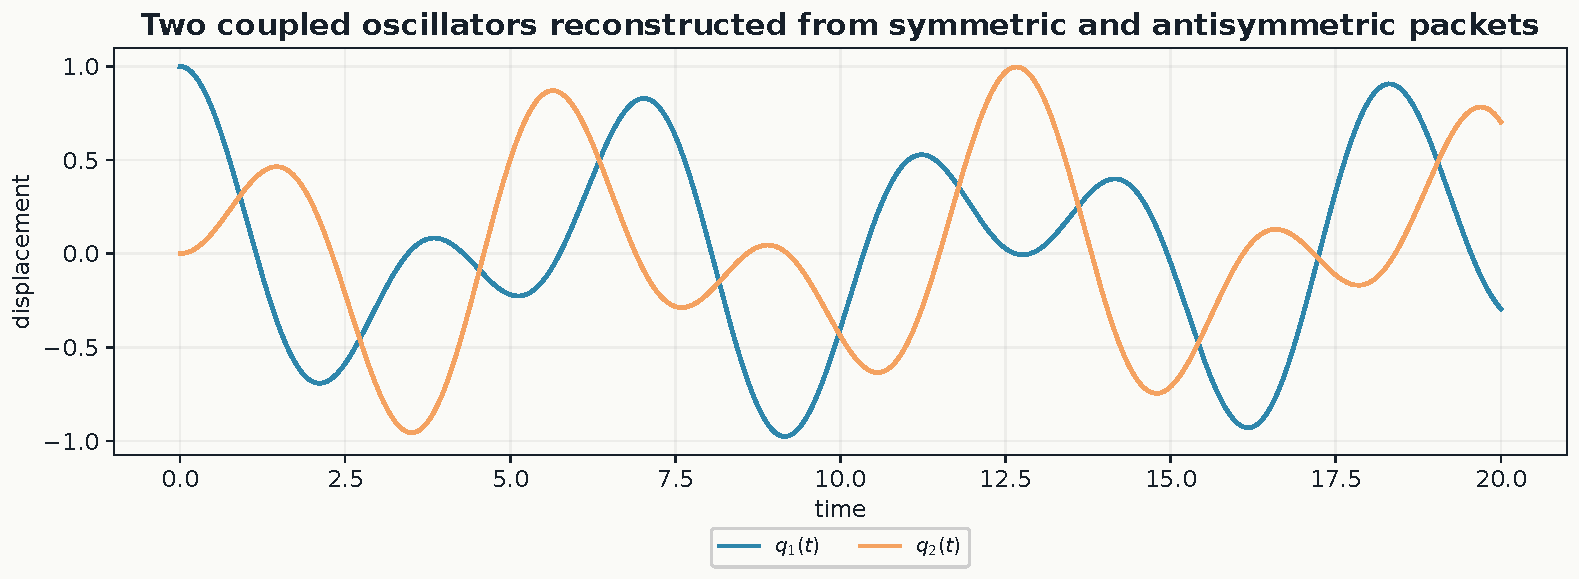
\includegraphics[width=.90\linewidth]{14_coupled_oscillator_motion.pdf}
\caption{The physical coordinates reconstructed from the two normal-mode packets. The legend is placed below the axes so it cannot cover the trajectories.}
\end{figure}

\SafeFigure[.97\linewidth]{34_physics_modal_reconstruction.pdf}{Top row: modal coordinates and reconstructed physical coordinates. Bottom row: the two closed phase-space orbits, each generated by one conserved modal energy.}{fig:physics-modal-reconstruction}

\section{Step 3: verify the equation}
First verify the initial data. At $t=0$,
\[
q(0)=P_sq_0+P_aq_0=(P_s+P_a)q_0=q_0,
\]
and
\[
q'(0)=P_sv_0+P_av_0=v_0.
\]
Now differentiate twice. Since
\[
KP_s=P_s,
\qquad
KP_a=3P_a,
\]
we obtain
\[
q''(t)=-P_sq(t)-3P_aq(t)=-Kq(t).
\]
The symbolic residual $q''+Kq$ is the zero vector.

\section{Step 4: energy packets}
The total energy is
\[
E(t)=\frac12\norm{q'(t)}^2+\frac12q(t)^{\mathsf T}Kq(t).
\]
Because the packet spaces are orthogonal and $K=P_s+3P_a$,
\[
E=E_s+E_a,
\]
where
\[
E_s=\frac12\norm{P_sq'}^2+\frac12\norm{P_sq}^2,
\]
and
\[
E_a=\frac12\norm{P_aq'}^2+\frac32\norm{P_aq}^2.
\]
For the chosen initial condition,
\[
E_s(0)=\frac12\norm{P_sq_0}^2
=\frac12\left(\frac12\right)=\frac14,
\]
while
\[
E_a(0)=\frac32\norm{P_aq_0}^2
=\frac32\left(\frac12\right)=\frac34.
\]
Therefore
\[
\boxed{E_s=\frac14,
\qquad E_a=\frac34,
\qquad E=1.}
\]
All three quantities are independent of time.  The total conservation law is not checked only at $t=0$: symbolic differentiation and simplification prove $dE/dt=0$ identically.

\begin{figure}[H]
\centering
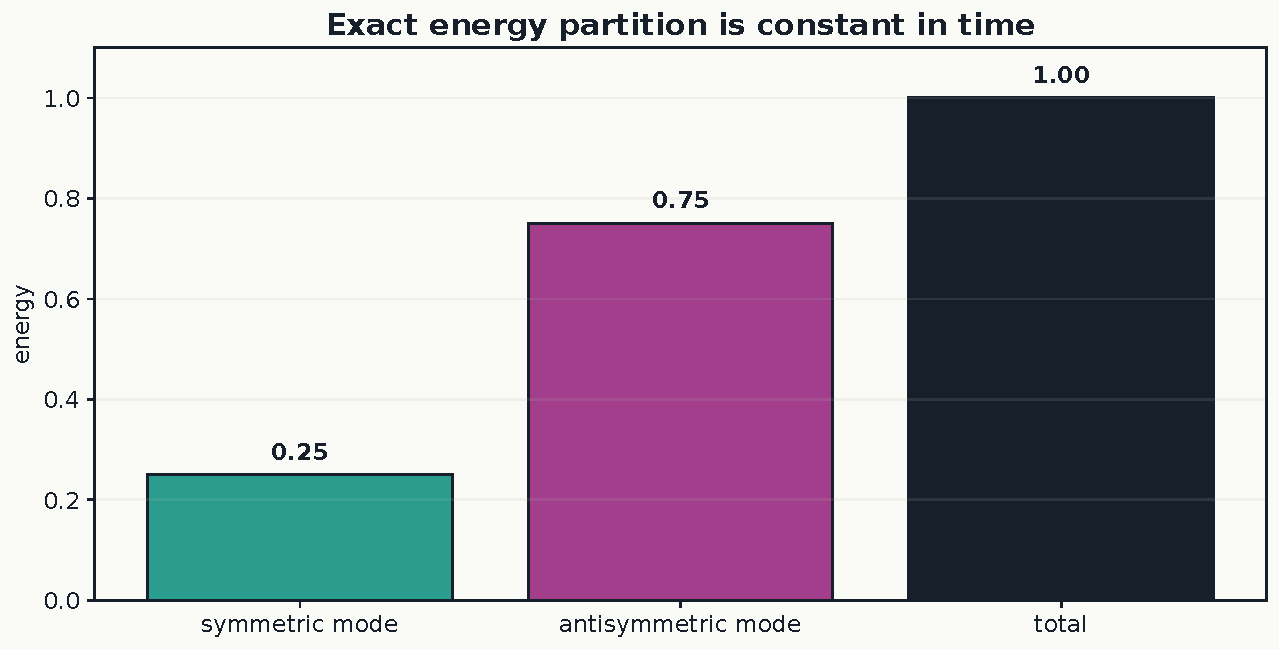
\includegraphics[width=.72\linewidth]{15_coupled_oscillator_energy.pdf}
\caption{The symmetric and antisymmetric packet energies add to the conserved total.}
\end{figure}

\begin{certificate}
SymPy simplifies
\[
P_s^2-P_s=0,
\quad
P_a^2-P_a=0,
\quad
P_sP_a=0,
\quad
K-P_s-3P_a=0,
\]
\[
q''(t)+Kq(t)=0,
\quad
E(t)-1=0,
\quad
E_s-\frac14=0,
\quad
E_a-\frac34=0.
\]
\end{certificate}

\chapter{Area VII: nonlinear packets and geometric holonomy}\label{ch:nonlinear}

\section{Part A: nonlinear signal packets}
Consider the periodic memory-one nonlinear filter
\[
y[n]=x[n]+\frac12x[n-1]^2.
\]
Use the input
\[
x=(1,2,0,-1,3,1,-2,2)^{\mathsf T}.
\]
Define even and odd channels
\[
e[k]=x[2k],
\qquad
o[k]=x[2k+1].
\]
For the chosen signal,
\[
e=(1,0,3,-2)^{\mathsf T},
\qquad
o=(2,-1,1,2)^{\mathsf T}.
\]
Then the exact output packets are
\[
\boxed{y_e[k]=e[k]+\frac12o[k-1]^2,}
\]
\[
\boxed{y_o[k]=o[k]+\frac12e[k]^2.}
\]
Evaluating the two packet formulas gives
\[
y_e=\left(3,2,\frac72,-\frac32\right)^{\mathsf T},
\qquad
y_o=\left(\frac52,-1,\frac{11}2,4\right)^{\mathsf T}.
\]
For example,
\[
y_e[0]=e[0]+\frac12o[-1]^2
=1+\frac12(2)^2=3,
\]
and
\[
y_o[2]=o[2]+\frac12e[2]^2
=1+\frac12(3)^2=\frac{11}{2}.
\]
Interleaving these two channels yields
\[
y=\left(3,\frac52,2,-1,\frac72,\frac{11}2,-\frac32,4\right)^{\mathsf T},
\]
which agrees exactly with direct nonlinear filtering.

\SafeFigure[.94\linewidth]{35_nonlinear_channel_values.pdf}{The even and odd input packets and the two exact nonlinear output packets. All four coordinates in each channel are shown explicitly.}{fig:nonlinear-channel-values}

\begin{proof}
At even address $n=2k$, the previous periodic address is $2k-1$, which lies in the odd channel at packet index $k-1$. At odd address $n=2k+1$, the previous address is $2k$, which lies in the even channel at index $k$. Substitution gives the two displayed formulas. Interleaving restores every output address.
\end{proof}

\begin{figure}[H]
\centering
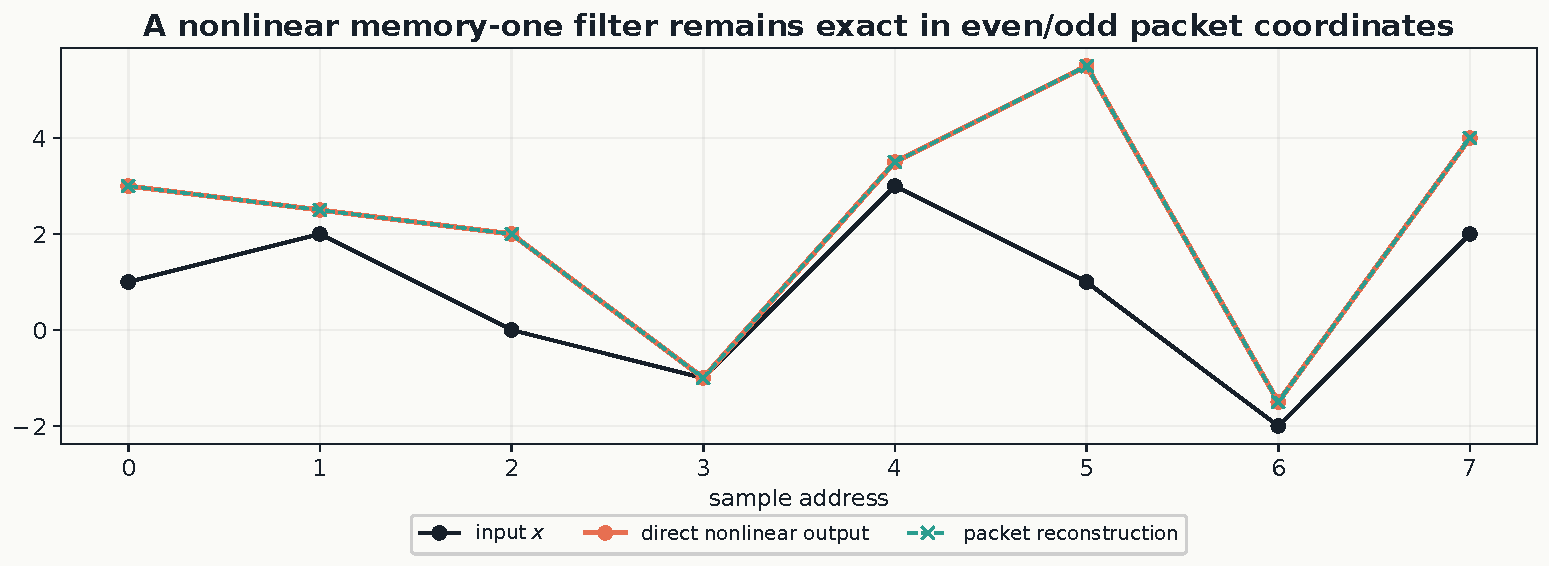
\includegraphics[width=.90\linewidth]{16_nonlinear_filter_packets.pdf}
\caption{Direct nonlinear filtering and packetwise reconstruction coincide.}
\end{figure}

\section{Part B: a finite gauge-gluing problem}
Let a directed square have vertices $v_0,v_1,v_2,v_3$. Suppose one edge system is trivial and a second is produced by vertex gauges $U_v$:
\[
B_{vu}=U_vU_u^{-1}.
\]
Choose rational orthogonal matrices
\[
U_0=I,
\quad
U_1=\begin{pmatrix}3/5&-4/5\\4/5&3/5\end{pmatrix},
\]
\[
U_2=\begin{pmatrix}5/13&-12/13\\12/13&5/13\end{pmatrix},
\quad
U_3=\begin{pmatrix}7/25&-24/25\\24/25&7/25\end{pmatrix}.
\]

The four exact edge transports are
\[
B_{10}=\begin{pmatrix}3/5&-4/5\\4/5&3/5\end{pmatrix},
\qquad
B_{21}=\begin{pmatrix}63/65&-16/65\\16/65&63/65\end{pmatrix},
\]
\[
B_{32}=\begin{pmatrix}323/325&-36/325\\36/325&323/325\end{pmatrix},
\qquad
B_{03}=\begin{pmatrix}7/25&24/25\\-24/25&7/25\end{pmatrix}.
\]
Each is orthogonal with determinant one because it is a rational rotation. Their entries are exact rational numbers, not decimal approximations.

\SafeFigure[.98\linewidth]{36_holonomy_edge_matrices.pdf}{The four rational edge-transport matrices. The common color scale makes their signs and magnitudes directly comparable.}{fig:holonomy-edge-matrices}

The cycle holonomy is
\[
H=B_{03}B_{32}B_{21}B_{10}.
\]
Telescoping gives
\[
H=U_0U_3^{-1}U_3U_2^{-1}U_2U_1^{-1}U_1U_0^{-1}=I.
\]

\begin{figure}[H]
\centering
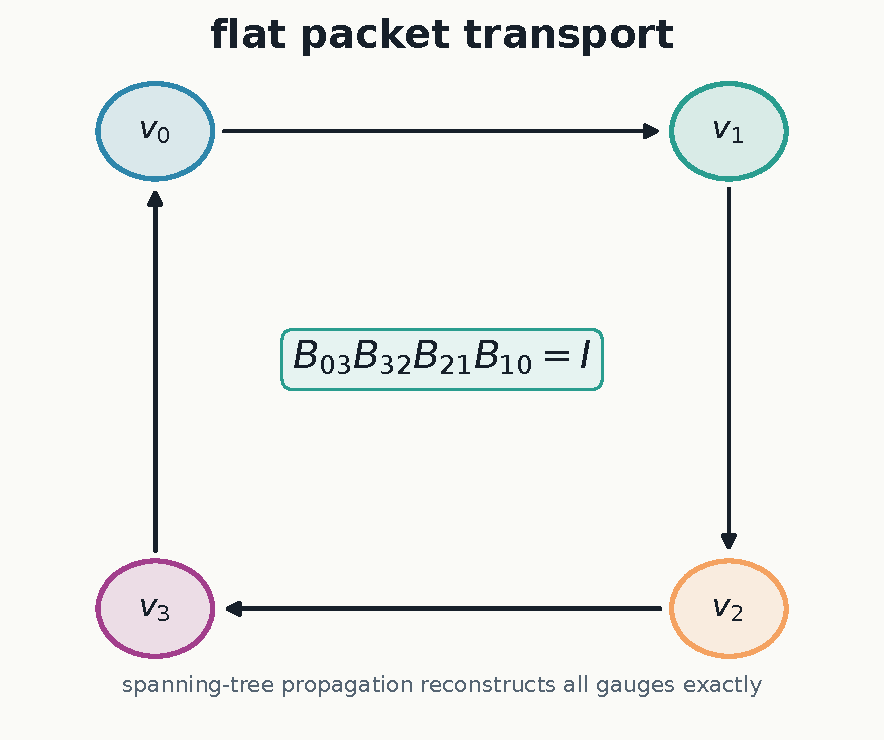
\includegraphics[width=.66\linewidth]{17_flat_holonomy.pdf}
\caption{A flat packet transport system on one fundamental cycle.}
\end{figure}

\begin{theorem}[Finite cycle obstruction]
Fix a root gauge and propagate gauges along a spanning tree. A global gauge exists on the whole connected graph if and only if every non-tree edge closes with the required fundamental-cycle holonomy.
\end{theorem}

\begin{proof}
Tree propagation determines every vertex gauge uniquely from the root. Each omitted edge imposes one remaining consistency equation. Multiplying that edge equation with the tree path gives the fundamental-cycle holonomy condition. Conversely, if every such cycle closes, all omitted edge equations hold.
\end{proof}

\section{Negative control}
Perturb the closing edge by left multiplication with
\[
Q=\begin{pmatrix}3/5&-4/5\\4/5&3/5\end{pmatrix},
\qquad
B_{03}^{\mathrm{bad}}=QB_{03}.
\]
Then
\[
H_{\mathrm{bad}}
=B_{03}^{\mathrm{bad}}B_{32}B_{21}B_{10}
=Q(B_{03}B_{32}B_{21}B_{10})=Q.
\]
The new holonomy is exactly $Q$, not $I$. The obstruction packet is
\[
H-I=
\begin{pmatrix}-2/5&-4/5\\4/5&-2/5\end{pmatrix}.
\]
Its squared Frobenius norm is
\[
\begin{aligned}
\norm{H-I}_F^2
&=\left(-\frac25\right)^2+\left(-\frac45\right)^2
+\left(\frac45\right)^2+\left(-\frac25\right)^2\\
&=\frac4{25}+\frac{16}{25}+\frac{16}{25}+\frac4{25}
=\boxed{\frac85}.
\end{aligned}
\]
This nonzero residual proves that no gauge satisfying all four perturbed edge equations exists with the chosen root normalization.

\begin{figure}[H]
\centering
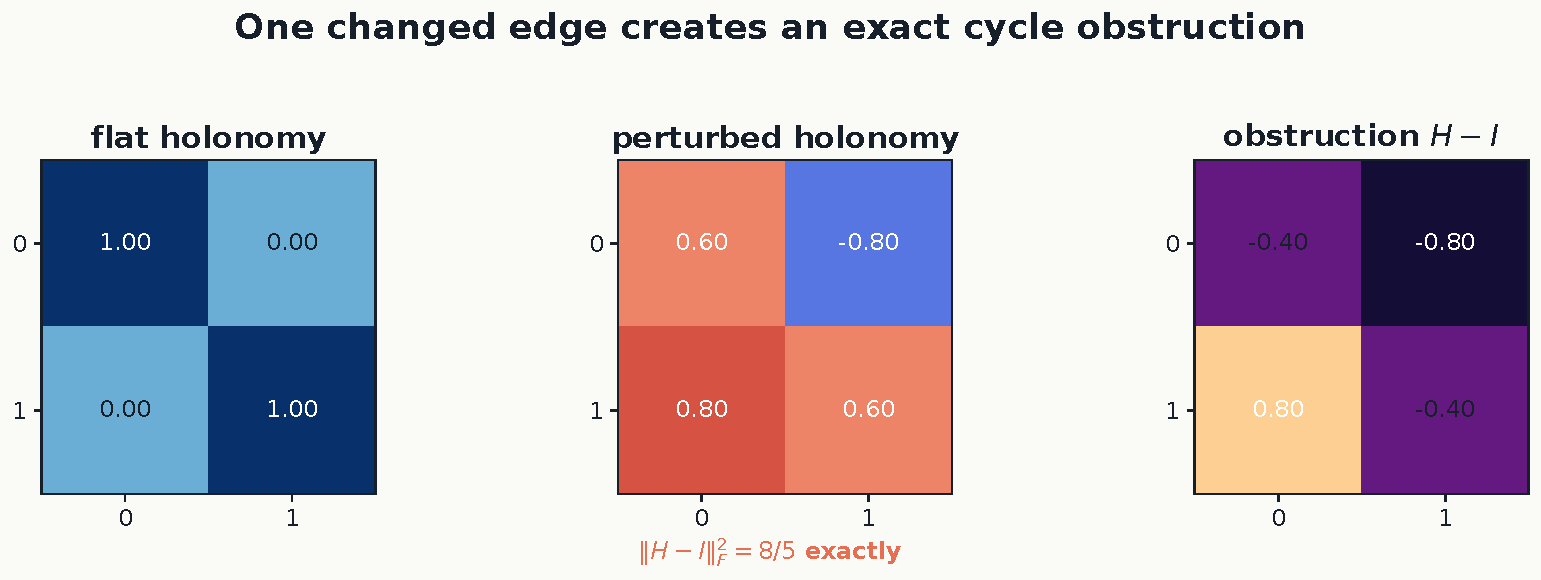
\includegraphics[width=.88\linewidth]{18_holonomy_obstruction.pdf}
\caption{Flat holonomy, perturbed holonomy, and the exact obstruction matrix.}
\end{figure}

\begin{certificate}
The nonlinear reconstruction residual is exactly zero. The flat cycle residual is exactly zero. The perturbed cycle returns the rational rotation $Q$ exactly, and the obstruction norm squared simplifies to $8/5$.
\end{certificate}

\part{Cross-Domain Synthesis}

\chapter{What the seven examples prove}\label{ch:synthesis}

\section{One theorem schema, seven domain meanings}
\small\begin{longtable}{L{0.82in}L{1.02in}L{1.16in}L{1.43in}L{1.45in}}
\caption{The same finite grammar in seven domains.}\\
\toprule
Area & Object & Packets & Transfer/refinement & Reconstruction \\
\midrule
\endfirsthead
\toprule
Area & Object & Packets & Transfer/refinement & Reconstruction \\
\midrule
\endhead
Linear algebra & vector or matrix & coordinate subspaces & matrix corners & sum of packets/blocks \\
Signals & sampled signal & phases, bands, Haar coordinates & polyphase and transform maps & interleaving or inverse transform \\
Quantum & state or density matrix & parity/basis sectors & gate path blocks & coherent path sum \\
Probability & observable or prior & partition cells & conditional expectation/Bayes update & packet masses and posterior \\
Arithmetic & analytic seed & exponent residue classes & differentiation, reciprocal powers & block-EGF coefficient synthesis \\
Physics & displacement field & normal modes & modal evolution & sum of mode solutions \\
Nonlinear geometry & nonlinear signal or edge system & phase packets/cycle packets & nonlinear interaction and holonomy & interleaving or global gauge \\
\bottomrule
\end{longtable}

\section{Seven-realization certificate}
\begin{theorem}[Cross-domain finite validity]
Each of Chapters~\ref{ch:linear}--\ref{ch:nonlinear} supplies a finite complete packet system or an explicitly invertible analysis-synthesis pair. In each case:
\begin{enumerate}[label=(\roman*)]
\item the declared packet identities hold;
\item the domain operator or map has an exact packet form;
\item the domain problem is solved at packet level;
\item synthesis reproduces the full object or solution;
\item an independent symbolic computation verifies the identity.
\end{enumerate}
Therefore Projector-Resolved Seed Calculus is a valid common finite calculus for these seven realizations.
\end{theorem}

\begin{proof}
The hypotheses and certificates are established separately in the seven chapters. The conclusion is their conjunction. No cross-domain analogy is used as a substitute for any domain proof.
\end{proof}

\SafeFigure[.94\linewidth]{37_cross_domain_proof_matrix.pdf}{Every area completes all five stages of the protocol: packet declaration, analysis, transfer or refinement, synthesis, and an independent audit.}{fig:cross-domain-proof-matrix}

\begin{figure}[H]
\centering
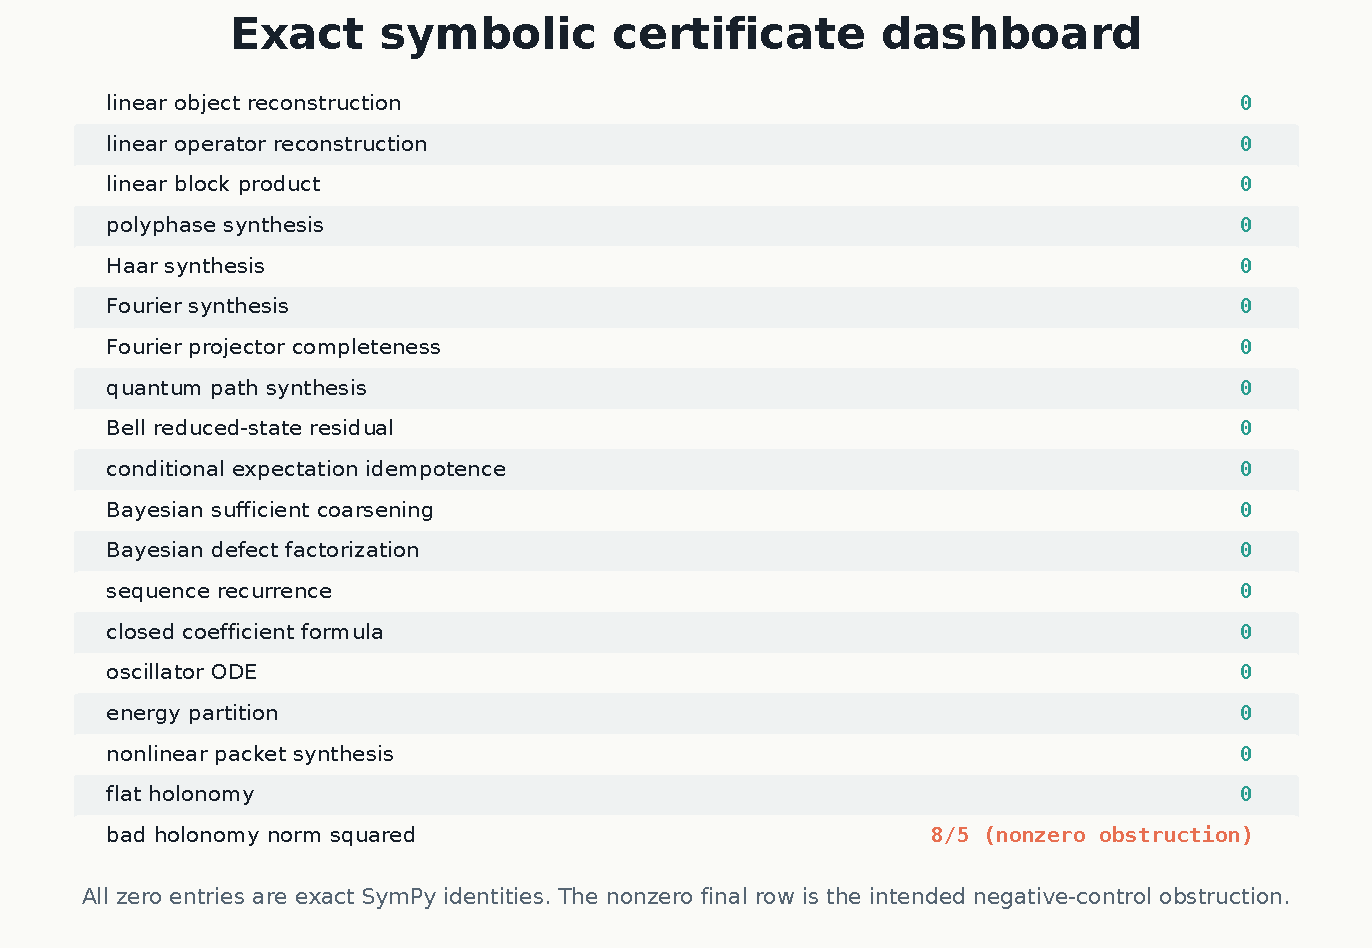
\includegraphics[width=.92\linewidth]{19_verification_dashboard.pdf}
\caption{All intended exact residuals vanish. The final nonzero row is the designed holonomy obstruction.}
\end{figure}

\section{Why this is stronger than a list of examples}
The examples do not merely reuse the words ``packet'' and ``reconstruction.'' They instantiate the same algebraic statements:
\[
\sum_\alpha P_\alpha=I,
\qquad
x=\sum_\alpha P_\alpha x,
\qquad
T=\sum_{\alpha,\beta}P_\beta TP_\alpha,
\]
with domain-specific meanings for $X$, $P_\alpha$, and $T$. The signal and quantum chapters use unitary coordinate transport; the Bayesian chapter uses nonlinear normalization after a linear packet map; the arithmetic chapter uses coefficient projectors and analytic completion; the physics chapter uses spectral projectors; and the holonomy example uses cycle packets as exact obstruction coordinates.

\section{What remains outside this document}
The following are not consequences of seven finite worked realizations:
\begin{itemize}
\item universal existence of preferred or optimal packets;
\item automatic continuum limits for unbounded operators;
\item universal recovery of hidden signal boundaries;
\item general quantum-spacetime dynamics;
\item unrestricted arithmetic or automorphic reciprocity;
\item historical priority for every generated special-function family.
\end{itemize}
Those questions require additional hypotheses and separate theorems. The value of this volume is that the finite core has now been proved, instantiated, solved, and computationally audited in seven genuinely different settings.

\appendix

\part{Appendices}

\chapter{Exact result ledger}
\begin{longtable}{L{2.15in}L{1.15in}L{2.75in}}
\caption{Machine-checked identities.}\\
\toprule
Certificate & Exact value & Interpretation \\
\midrule
\endfirsthead
\toprule
Certificate & Exact value & Interpretation \\
\midrule
\endhead
Linear object reconstruction & $0$ & Complete packet synthesis \\
Linear operator reconstruction & $0$ & Sum of transfer blocks \\
Linear product law & $0$ & Matrix multiplication through packet paths \\
Linear refinement & $0$ & Parent equals child sum \\
Polyphase synthesis & $0$ & Exact interleaving \\
Haar reconstruction & $0$ & Orthogonal filter-bank synthesis \\
Fourier reconstruction & $0$ & Unitary inverse DFT \\
Fourier projector completeness & $0$ & Complete band cover \\
Quantum path synthesis & $0$ & Bell state from two packet paths \\
Quantum reduced-state residual & $0$ & $\rho_A=I/2$ \\
Conditional-expectation idempotence & $0$ & Finite stochastic projector \\
Weighted self-adjointness & $0$ & Orthogonality in $L^2(\mu)$ \\
Sufficient Bayesian coarsening & $0$ & Conditioning commutes with coarsening \\
Bayesian defect factorization & $0$ & Exact information-loss packet \\
Sequence recurrence & $0$ & Every computed term satisfies the recurrence \\
Reciprocal-series product & $0$ & $D_5^2S=1$ in the computed block range \\
Hypergeometric coefficient identity & $0$ & Factorial multiplication formula \\
Composition coefficient formula & $0$ & Independent finite formula \\
Oscillator ODE residual & $0$ & Exact physical solution \\
Energy partition residual & $0$ & $E=E_s+E_a$ \\
Nonlinear filter residual & $0$ & Exact nonlinear packet synthesis \\
Flat holonomy residual & $0$ & Gauge system glues \\
Perturbed holonomy obstruction & $8/5$ & Intended nonzero negative control \\
Linear contribution-row reconstruction & $0$ & Three block contributions sum to each output packet \\
Fourier band-signal reconstruction & $0$ & Five pulled-back band packets sum to the signal \\
Complete quantum path table & exact & Two nonzero and two zero parity paths \\
Bayesian same-coarse-prior witness & $(6/145,-6/145)$ & Nonsufficiency produces distinct coarse posteriors \\
Arithmetic recurrence rows $1$--$4$ & exact & Two integer contributions sum to each coefficient \\
Normal-mode orthogonality & $0$ & Spectral packet basis is orthonormal \\
Holonomy edge product & $I_2$ & Four rational transports close exactly \\
\bottomrule
\end{longtable}

\chapter{Candidate OEIS submission record}
\section*{Name}
Order-five reciprocal-square generalized Euler packet numbers.

\section*{Definition}
\[
\sum_{n\ge0}a_n\frac{z^{5n}}{(5n)!}
=
\left(
\sum_{n\ge0}(-1)^n\frac{z^{5n}}{(5n)!}
\right)^{-2}.
\]

\section*{Initial terms}
\begin{longtable}{rL{5.4in}}
\toprule
$n$ & $a_n$ \\
\midrule
0 & 1 \\
1 & 2 \\
2 & 754 \\
3 & 3009008 \\
4 & 58105670266 \\
5 & 3690819041733782 \\
6 & \texttt{\seqsplit{611297487195595912564}} \\
7 & \texttt{\seqsplit{225925381294863591587930378}} \\
8 & \texttt{\seqsplit{166595785020134064487394817914506}} \\
9 & \texttt{\seqsplit{225274815520247848148603077637197668512}} \\
10 & \texttt{\seqsplit{522980674085092488996787781136498102984642274}} \\
11 & \texttt{\seqsplit{1976933475656337920957015185269270006672342520220798}} \\
12 & \texttt{\seqsplit{11650813481135176558042711997383235316672795614675522384596}} \\
\bottomrule
\end{longtable}

\section*{Formula}
The recurrence and closed form are those proved in Chapter~\ref{ch:arithmetic}. The machine-readable b-file is supplied as \texttt{tables/candidate\_sequence\_bfile.txt}.

\section*{Status}
OEIS-ready candidate record. The exact definition, recurrence, initial values, and b-file are supplied. No historical-priority or database-absence claim is used in the mathematics.

\chapter{Reproduction commands}
From the extracted source directory:
\begin{lstlisting}[language=bash]
python -m pip install -r requirements.txt
python -m pytest -q
python run_all.py
python -m pytest -q
latexmk -pdf Seven_Area_Worked_Proof_Atlas.tex
\end{lstlisting}
The command \texttt{python run\_all.py} regenerates all sixty-one figure pairs, every CSV table, the candidate b-file, and the JSON result ledger. The test suite contains thirty-two exact tests: eleven seed-to-reconstruction foundation tests, seven primary domain certificates, seven independent re-derivations, and seven additional audits of the detailed intermediate calculations.

\chapter{Full symbolic source listings}
The following listings are the complete exact calculation modules used in the release.

\section{Seed-to-reconstruction foundations}
\lstinputlisting{proof_atlas/foundations.py}

\section{Foundation figure generator}
\lstinputlisting{proof_atlas/foundation_figures.py}

\section{Finite linear algebra}
\lstinputlisting{proof_atlas/linear.py}

\section{Signals and transform atlases}
\lstinputlisting{proof_atlas/signal.py}

\section{Quantum circuit}
\lstinputlisting{proof_atlas/quantum.py}

\section{Conditional expectation and Bayesian refinement}
\lstinputlisting{proof_atlas/bayes.py}

\section{Arithmetic root-filter sequence}
\lstinputlisting{proof_atlas/arithmetic.py}

\section{Coupled oscillators}
\lstinputlisting{proof_atlas/physics.py}

\section{Nonlinear packets and holonomy}
\lstinputlisting{proof_atlas/nonlinear_geometry.py}

\section{Detailed intermediate certificates}
\lstinputlisting{proof_atlas/details.py}

\section{Seed-to-reconstruction foundation tests}
\lstinputlisting{tests/test_foundations.py}

\section{Implementation-certificate tests}
\lstinputlisting{tests/test_proofs.py}

\section{Independent re-derivation audit}
\lstinputlisting{tests/test_z_independent_audit.py}

\section{Detailed derivation audits}
\lstinputlisting{tests/test_detailed_derivations.py}

\chapter{Layout and figure audit}
The complete seed-to-reconstruction edition treats page fit as a reproducibility condition. Every figure is exported in vector PDF and high-resolution PNG form. The final PDF is rendered page by page, and the audit checks the following:
\begin{enumerate}[label=(\roman*)]
\item no legend covers plotted data;
\item every plot title, axis label, and tick label remains inside the figure boundary;
\item diagram labels are conservatively sized for their boxes;
\item each included figure is constrained by both page width and page height;
\item captions use ragged-right paragraph layout rather than overflowing single lines;
\item no LaTeX overfull or underfull boxes remain in the final build.
\end{enumerate}
The machine-readable layout report is included in \texttt{results/layout\_audit.json}.

\chapter{Source and claim map}
\begin{tabularx}{\linewidth}{L{1.6in}Y Y}
\toprule
Layer & Source & Role \\
\midrule
Seed-to-finish calculus & Chapters~\ref{ch:seed-first}--\ref{ch:start-finish-theorem} & Proves generation, relations, packets, transfer, paths, refinement, atlases, nonlinear coordinates, obstructions, completion, and final reconstruction \\
Domain mathematics & Chapters~\ref{ch:linear}--\ref{ch:nonlinear} & Retains all seven original worked problems and their detailed derivations \\
Symbolic implementation & \texttt{proof\_atlas/*.py} & Independent exact computation \\
Tests & \path{tests/test_foundations.py} and the three retained domain test modules & Eleven foundational tests plus twenty-one retained domain tests \\
Figures & \texttt{figures/} & Visual explanations generated from exact data \\
Tables/results & \texttt{tables/}, \texttt{results/} & Machine-readable values and residuals \\
OEIS note & arithmetic chapter and candidate record & Candidate status only; no unconditional novelty claim \\
\bottomrule
\end{tabularx}

\chapter{Conclusion}
The complete seed-to-reconstruction content of Projector-Resolved Seed Calculus can be stated without metaphor:
\[
\boxed{
\begin{gathered}
\text{seed and fixed grammar}
+\text{relations and complete packets}
+\text{typed transfer and nonlinear interaction}\\[2pt]
+\text{compatible refinement and declared completion}
+\text{declared synthesis}\\[2pt]
=\text{exact reconstruction}.
\end{gathered}
}
\]
The seven worked areas show the same identity operating on vectors, signals, quantum states, probability models, analytic coefficient families, mechanical modes, nonlinear filters, and gauge transports. The examples differ in meaning and technique, but they share a single finite grammar. That grammar has now been proved abstractly, realized concretely, and checked symbolically from beginning to end.

\end{document}
